\documentclass[11pt,a4paper]{article}
\usepackage[margin=1in]{geometry}
\usepackage{amsmath,amssymb}
\usepackage{graphicx}
\usepackage{booktabs}
\usepackage{longtable}
\usepackage{xcolor}
\usepackage[hidelinks]{hyperref}
\usepackage{caption}

\newcommand{\code}[1]{\texttt{\small #1}}
\newcommand{\elmax}{\ensuremath{\ell_{\max}}}
\newcommand{\lammin}{\ensuremath{\lambda_{\min}}}
\newcommand{\zetav}{\ensuremath{\zeta}}
\captionsetup{font=small,labelfont=bf}

% File paths set in typewriter do not hyphenate, so long \code{...} spans
% overflow the measure. Allow the paragraph builder to stretch inter-word
% space instead; this is a technical note, not a typeset book.
\sloppy

\usepackage{bm}


\title{\bf The Order-2 FK term in the lensing two-point function:\\
a numerical audit and corrected results}
\author{}
\date{2026 August}

\begin{document}
\maketitle

\begin{abstract}
\noindent
The Order-2 ``FK'' contribution plotted in the draft is not a faithful
evaluation of the quantity the draft defines. The three-point driving-field
vertex it needs is tabulated on a cosine mesh whose only samples on the
relevant family are at zero separation and at $31^\circ$, so over the whole
plotted range the vertex lookup returns the zero-separation value. The
published curve's angular dependence reproduces the interpolator's weight
function to one part in $10^4$, evidence internal to the deployed files.
The amplitude at arcminute separations survives, to $0.15\%$; the shape does
not, being overstated by factors of $5$ at $22'$ and $100$ at $114'$ and
carrying the wrong sign beyond $230'$. Corrected, the FK term stays a small
fraction of Order-0 at every separation instead of overtaking it near
$2^\circ$, and it appears in $\xi_-$ and $\xi_{\kappa\gamma}$ at a
comparable level instead of vanishing.

Three further results are independent of that correction. The multipole
cutoff of the vertex build is not converged: the tree-level integral turns
over near $\ell\sim10^4$, an order of magnitude above the deployed value,
and carrying it there raises the arcminute amplitude from $0.5\%$ of
Order-0 to $2.31\%$. Replacing the tree-level bispectrum by BiHalofit
does not converge at all, and not because the sum was stopped too early:
the FK term samples a coincident-point moment, which is ultraviolet
sensitive by construction and has a finite value only because the linear
spectrum happens to be steep enough. With a nonlinear spectrum it has no
limit, and the formalism supplies no smoothing scale to give it one, so the
cutoff acts as an unstated regulator and the nonlinear FK term reaches
$41\%$ of Order-0. A finite beam width would supply the missing scale, and
the algebra of that proposal is verified here; which scale to adopt is a
choice about the observable that remains open. The absolute
normalisation, by contrast, is correct: the pipeline's own factor chain
reduces to the standard Limber convergence bispectrum with ratio unity to
machine precision. And the equal-split claim
$\Delta C_\ell^{EE}=\Delta C_\ell^{BB}$ is a coincident-limit identity:
away from coincidence the two polarizations separate and the E-mode comes to
dominate, the B-mode falling from $0.95$ of the E-mode power at $\ell=60$ to
$0.42$ at $\ell=1500$.

This note reports the measurements, the corrected figures, and the specific
statements in the draft that do and do not survive.
Section~\ref{sec:afterwards} records four findings that came later, while the
revision was being carried out, and that changed what was done: the FK
Monte-Carlo does not measure the FK diagram; the multi-redshift FF slices had
never been computed; the multipole sum stops converging beyond about a degree,
which bounds where FK may be quoted; and the $\zeta$-slices figure was still
drawn at the old cutoff.
\end{abstract}

\tableofcontents

\section{What was checked, and how}
\label{sec:scope}

This note reports a numerical audit of the Order-2 ``FK'' contribution to
the lensing two-point function, the term the draft plots in
\code{figures/analysis3\_NLO\_FFFK.pdf} and
\code{figures/analysis3\_cl\_full\_vs\_O0.pdf} and quotes in
\code{sections/insights.tex} and \code{sections/conclusion.tex}.

Six questions were asked, in this order.

\begin{enumerate}
\item Does the plotted FK curve evaluate the quantity the paper defines?
      (Section~\ref{sec:sampling})
\item Is the multipole cutoff in the vertex build converged, and if not,
      what does the converged answer rest on? (Section~\ref{sec:cutoff})
\item Does the line-of-sight floor $\lammin$ of the tabulated vertex bias
      the result, and does the bias depend on source redshift?
      (Section~\ref{sec:lambdamin})
\item Is the absolute normalisation of the vertex right, having never been
      compared against anything external? (Section~\ref{sec:normalisation})
\item Do the draft's statements about the E and B polarization structure
      survive a resolved vertex? (Section~\ref{sec:eb})
\item Does a nonlinear bispectrum give a more realistic prediction?
      (Section~\ref{sec:nonlinear}), and if the answer is no, what exactly
      is missing? (Section~\ref{sec:uv})
\end{enumerate}

The first is the one that changes published numbers. The fourth is the one
whose answer is unreservedly positive. The rest fall in between.

The first was settled by an independent reviewer who was given the figure
production path and nothing else. That reviewer was not told what any
earlier work had concluded, was blocked from reading the earlier notes, and
was told explicitly that finding nothing wrong would be a useful result. It
worked forward from the figure manifest through the generator scripts, the
folded \code{xi\_*.npz} files, the run configuration, the vertex callable
and the tabulated vertex, testing rather than assuming at each step. Its
conclusion agreed with the earlier work, and it added several results the
earlier work did not have. The comparison is recorded in
\code{notes/task\_a\_blind\_audit\_comparison.md}.

Two controls make the rest of the note interpretable.

\paragraph{The pipeline is reproducible.} Re-running the production FK fold
from a redirected copy of its own configuration reproduces the deployed
result bit for bit, with maximum relative difference zero across all six
component pairs. Every comparison below therefore isolates exactly one
change.

\paragraph{The rebuild machinery is exact.} The vertex table is rebuilt
here in pieces: one radial-and-multipole LOW branch, and a set of HIGH
multipole windows that are summed. This is only legitimate if the pieces
are independent, so that was tested rather than assumed. Table rows are
bit-exactly independent of one another in both branches: computing a row in
a table of six rows and in a table of two rows gives identical doubles
(\code{np.array\_equal} true, maximum relative difference $0.000$). The
multipole windows are disjoint in maximum leg, so their sum is the same
integral. Together these mean one build at the finest grid yields every
coarser grid by row selection, and every smaller cutoff by partial
summation, with no approximation. The reimplementation of the production
triple mesh reproduces the deployed table's 1671 rows exactly and in the
same order.

All commands are in \code{driver\_field\_emulators/code/}, and every number
quoted below names the script that produced it.

\section{The vertex sampling problem}
\label{sec:sampling}

This section rests entirely on the deployed table and the deployed folded
result. No rebuilt table is used, so none of it depends on trusting a
second calculation.

\subsection{What the fold asks for}

The FK two-point fold evaluates the driving-field three-point cumulant on
the collapsed configuration: two directions coincident, the third displaced
by the plotted separation $\gamma$. In the cosine coordinates the vertex
table is indexed by, that is the family $(1,\cos\gamma,\cos\gamma)$. This
was established from the code rather than the documentation, by wrapping
the production callable in a logging shim and running the production
configuration. Across 1\,990\,656 recorded evaluations the fold requests
exactly one sorted cosine triple per separation, and the three leg times
agree to $2\times10^{-13}$, confirming the equal-time collapse. That is the
object \code{sections/appendix.tex} defines in appendix
\emph{append: driving-field spectra}.

\subsection{Where the table has samples}

The deployed table is built on a uniform mesh of 15 cosines, spacing
$1/7$, triangle filtered to 1671 rows, which the callable canonicalises to
351 unique sorted triples. On the collapsed family the mesh therefore has
samples at
\[
  c=1 \;\;(\gamma = 0), \qquad
  c=6/7 \;\;(\gamma = 31.0^\circ = 1860'), \qquad
  c=5/7 \;\;(\gamma = 44.4^\circ), \;\ldots
\]
There is no sample between $\gamma=0$ and $\gamma=1860'$. The figures plot
$0.5'$ to $5000'$, that is $0.008^\circ$ to $83^\circ$. Thirty-five of the
forty plotted separations lie inside the first mesh gap.

The compression is worse than the gap width suggests, because the
interpolation variable is $\cos\gamma$ and $1-\cos\gamma \simeq
\gamma^2/2$. Measured as a fraction of the first interval $[6/7,1]$, the
plotted separations sit at $0.0000\%$ ($\gamma=0.5'$), $0.014\%$
($21.9'$), $0.62\%$ ($144.7'$) and $4.1\%$ ($372.2'$). Twenty-six of the
forty are within $1\%$ of the $c=1$ endpoint. Both endpoints of the
interval are exact table entries; the difficulty is that the plotted range
does not span the interval, it hides inside one end of it.

\subsection{The plotted curve is the interpolation weight}

The callable looks a query up with a \code{cKDTree} over the 351 unique
triples, taking the four nearest neighbours with inverse-distance weights.
Reconstructing that lookup and reading off the normalised weight the rule
places on the $(1,1,1)$ node gives a curve that can be compared directly
with the published FK curve, normalised to its own value at $0.5'$.

They are the same curve. Over the whole range in which the corner node is
in the neighbour set, $0.5'$ to $1535'$, the largest absolute difference is
$5.2\times10^{-5}$ and the largest relative difference is
$2.4\times10^{-4}$ (Figure~\ref{fig:weight}). The plotted angular
dependence of the FK term is the interpolator's weight function. No
property of the vertex enters it.

At $\gamma=1944'$ the corner node leaves the four-neighbour set altogether,
its weight becoming exactly zero, and the curve changes sign. That is
$32.4^\circ$, and it is the feature the caption of Figure~15 in
\code{sections/appendix.tex} describes as ``the sign change at
$\gamma\simeq32^\circ$''. The four neighbours that replace it are
$(1,\tfrac67,\tfrac67)$, $(\tfrac67,\tfrac67,\tfrac67)$,
$(1,\tfrac57,\tfrac57)$ and $(\tfrac67,\tfrac67,\tfrac57)$: one collapsed
configuration at $31^\circ$, one equilateral triangle and one scalene
triangle. The sign change is a change of neighbour set.

\begin{figure}[t]
\centering
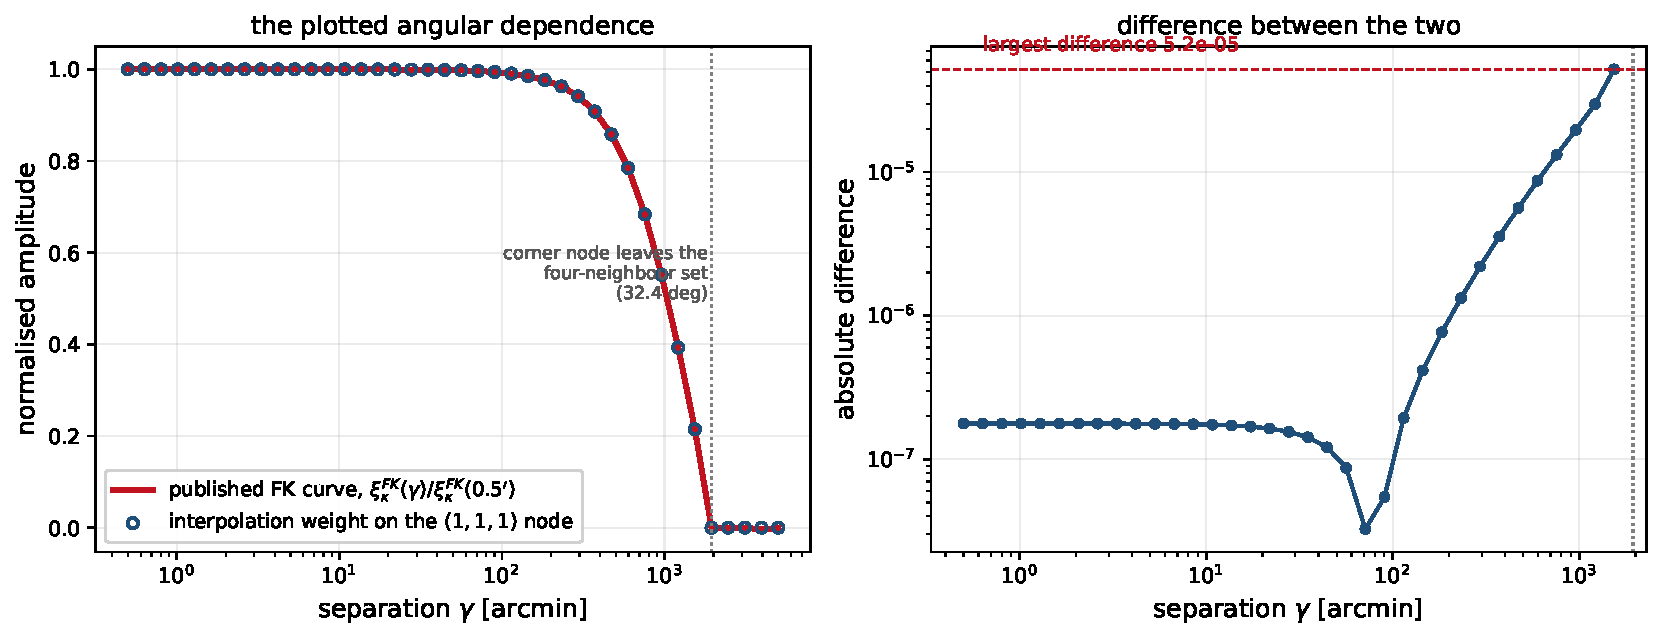
\includegraphics[width=\textwidth]{figures/weight_identity.pdf}
\caption{Left: the published FK curve for $\xi_\kappa$, normalised to its
value at $\gamma=0.5'$, against the normalised inverse-distance weight the
vertex callable places on the $(1,1,1)$ node. Right: the difference between
them. Both come from deployed artefacts only. The dotted line marks the
separation at which the corner node leaves the four-neighbour set, which is
where the published curve changes sign. Produced by
\code{code/rebuild/probe\_weight\_identity.py}.}
\label{fig:weight}
\end{figure}

\subsection{The deployed table's own next sample}

The table also says, by itself, that the vertex cannot be flat across this
range. On the source shell its collapsed-family entries read
$-1.35\times10^{-14}$ at $c=1$ and roughly three orders of magnitude
smaller, with the opposite sign, at $c=6/7$. The deployed file therefore
records that the vertex falls by more than three orders of magnitude and
changes sign somewhere inside the first gap. What it cannot record is
where.

There is an independent reason to expect the decay, which needs no table at
all. The collapsed configuration is the driving-field cumulant with two
points coincident and the third displaced transversely by $r_\perp =
\chi\gamma$ on the same shell. At the mid shell, $\gamma=0.5'$ is
$r_\perp\simeq1$ Mpc while $\gamma=145'$ is $r_\perp\simeq280$ Mpc. Matter
correlations die well before 280 Mpc, so the vertex must decay across the
plotted range. In the same units the mesh spacing of $1/7$ in $\cos\gamma$
is a resolution of about 3600 Mpc in $r_\perp$, while the physics happens
between 1 and 100 Mpc.

\subsection{The draft already contains the counterexample}

Figure~7 of the draft, \code{zeta\_driving\_field\_slices\_draft.pdf}, is
generated from \code{ell\_band\_decomp\_results.npz}, which evaluates the
vertex on the collapsed family at 28 separations directly, with no cosine
mesh and no interpolation. It shows the vertex decaying steeply and
changing sign inside the range over which the FK figures show it flat. The
two figures in the same paper disagree, and the resolved one is right.

\subsection{A second, smaller defect in the same callable}

The callable sorts a query triple descending before lookup and then fills
the coupling tensor with the retrieved value in every index permutation.
Whether that is legitimate depends on the channel. Building the same
collapsed configuration in the two leg orderings that canonicalise to the
same sorted triple, and comparing, gives the median relative differences in
Table~\ref{tab:perm}.

\begin{table}[h]
\centering
\begin{tabular}{lcc}
\toprule
channel & median relative difference & symmetric \\
\midrule
$\zeta_{TTT}$  & $3.3\times10^{-3}$ & yes \\
$\zeta_{Bmod}$ & $3.3\times10^{-3}$ & yes \\
$\zeta_{PPP}$  & $4.9\times10^{-2}$ & no \\
$\zeta_{TPP}$  & $2.3\times10^{-1}$ & no \\
$\zeta_{TTP}$  & $5.9\times10^{-1}$ & no \\
$\zeta_{Dmod}$ & $7.0\times10^{-1}$ & no \\
\bottomrule
\end{tabular}
\caption{Sensitivity of each vertex channel to which leg carries the
offset, over separations up to $200'$. The two orderings canonicalise to
the same sorted triple, so the callable cannot distinguish them and the
difference bounds the error its symmetric fill makes. Maxima are not quoted
because every channel passes through zero in this range. Produced by
\code{code/rebuild/probe\_permutation.py}.}
\label{tab:perm}
\end{table}

The channels that carry $\xi_\kappa$ and $\xi_+$ are symmetric to the
quadrature level, so the symmetric fill costs those two observables
nothing. The channels that enter $\xi_-$ and $\xi_{\kappa\gamma}$ are not,
so those two can be quoted here as magnitudes and signs but not as precise
values. This did not affect the deployed numbers, because the deployed
lookup is pinned at $(1,1,1)$, which has no permutation duplicates. It
becomes live exactly when the grid is refined, which is why it is fixed
rather than merely noted: Section~\ref{sec:callablefix} reports the
correction and what it changes.

\section{The multipole cutoff}
\label{sec:cutoff}

\subsection{What the cutoff is}

The vertex is built in two branches: an exact Wigner-3j sum for
$\ell\le60$, and a flat-sky Limber integral above it, truncated at
$\elmax$. The deployed value is $\elmax=1000$. The question is whether the
truncated integral has converged, and if not, what the converged answer
depends on.

Sweeping the cutoff naively answers neither, for two reasons. A partial sum
that is climbing slowly over one decade is indistinguishable from a
divergent one. And the deployed quadrature maps a fixed number of
Gauss-Legendre nodes linearly onto $[\ell_{\min},\elmax]$, so raising the
cutoff at fixed node count silently coarsens the rule and mixes truncation
with a resolution artefact.

Both are avoided by integrating in octave windows, each with its own
96-node rule. The windows are disjoint in maximum leg, so their sum is the
same integral, the node density per octave is fixed by construction, and
the partial sum up to any octave edge is the vertex built with that cutoff.
One band set therefore gives the whole curve.

\subsection{The integral converges, well above the deployed cutoff}

Table~\ref{tab:bands} gives the per-octave contribution at the source
shell, as a fraction of the total, together with the local slope $p$ from
fitting successive bands to $L^{-p}$. Positive $p$ means the tail is dying.

\begin{table}[h]
\centering
\begin{tabular}{lrrrrrr}
\toprule
& \multicolumn{3}{c}{$\gamma=0.5'$} & \multicolumn{3}{c}{$\gamma=21.9'$} \\
\cmidrule(lr){2-4}\cmidrule(lr){5-7}
band & contribution & fraction & $p$ & contribution & fraction & $p$ \\
\midrule
$(240,480]$    & $-4.19\times10^{-15}$ & 0.011 & $-3.04$ & $-1.46\times10^{-15}$ & 0.162 & $-1.89$ \\
$(480,960]$    & $-2.03\times10^{-14}$ & 0.055 & $-2.28$ & $+3.00\times10^{-16}$ & $-0.033$ & --- \\
$(960,1920]$   & $-5.57\times10^{-14}$ & 0.150 & $-1.46$ & $-1.92\times10^{-15}$ & 0.213 & --- \\
$(1920,3840]$  & $-9.69\times10^{-14}$ & 0.261 & $-0.80$ & $-2.20\times10^{-15}$ & 0.244 & $-0.20$ \\
$(3840,7680]$  & $-1.13\times10^{-13}$ & 0.303 & $-0.22$ & $-1.96\times10^{-15}$ & 0.217 & $+0.17$ \\
$(7680,15360]$ & $-8.14\times10^{-14}$ & 0.219 & $+0.47$ & $-1.49\times10^{-15}$ & 0.166 & $+0.39$ \\
\bottomrule
\end{tabular}
\caption{Octave-band contributions to $\zeta_{TTT}$ at the source shell,
tree level, on the corrected grid. The slope turns positive in the last
band at both separations, so the integral converges; it does so near
$\ell\sim10^4$, an order of magnitude above the deployed cutoff. The top
band still carries 17 to 22 percent of the total, so even $\elmax=15360$
is short of the converged value by roughly that much. Produced by
\code{code/rebuild/analyse\_cutoff.py}.}
\label{tab:bands}
\end{table}

So $\elmax$ is a numerical convergence parameter, not a physical smoothing
scale, and the deployed value of 1000 sits on the rising side of the
integrand, well below its peak. Relative to $\elmax=960$, the vertex at
$\gamma=0.5'$ on the source shell grows by

\begin{center}
\begin{tabular}{lrrrr}
\toprule
$\elmax$ & 1920 & 3840 & 7680 & 15360 \\
\midrule
tree      & 3.24 & 7.14 & 11.67 & 14.95 \\
BiHalofit & 3.26 & 7.33 & 12.90 & 18.99 \\
\bottomrule
\end{tabular}
\end{center}

\noindent
The two track each other to the first octave and then separate: by
$\elmax=15360$ the nonlinear vertex has grown by a further $27\%$ relative
to the tree one. That is the same statement as the slope table read the
other way. The nonlinear spectrum is flatter, so its turnover is later, and
its partial sum is still climbing where the tree one has begun to level
off.

The mechanism is the effective spectral slope. After the radial collapse
the hard pair contributes as a two-dimensional transverse integral
$\int\!\mathrm{d}k\,k\,P(k)$, whose integrand peaks where
$n_{\rm eff}=\mathrm{d}\ln P/\mathrm{d}\ln k$ equals $-1$ and which
converges once $n_{\rm eff}<-2$. The linear spectrum crosses $-2$ near
$k\simeq0.5\,h/$Mpc, so the tree vertex turns over at multipoles of order
$10^4$. The one-halo term flattens the nonlinear spectrum, pushing
$n_{\rm eff}$ back up to about $-1.1$ at $k\simeq1\,h/$Mpc, so the
nonlinear turnover is pushed much further out.

\subsection{The observable, as a function of the cutoff}

The vertex is not the observable. Folding each cutoff through the full
pipeline gives Table~\ref{tab:foldcut}.

\begin{table}[h]
\centering
\begin{tabular}{rrrr}
\toprule
$\elmax$ & $\xi^{\rm FK}_\kappa(0.5')$ & relative to $\elmax=960$ & as a fraction of Order-0 \\
\midrule
   960 & $+4.080\times10^{-6}$ & 1.00 & 0.48\% \\
  1920 & $+8.160\times10^{-6}$ & 2.00 & 0.97\% \\
  3840 & $+1.293\times10^{-5}$ & 3.17 & 1.53\% \\
  7680 & $+1.708\times10^{-5}$ & 4.19 & 2.02\% \\
 15360 & $+1.950\times10^{-5}$ & 4.78 & 2.31\% \\
\bottomrule
\end{tabular}
\caption{The folded FK contribution to $\xi_\kappa$ at the smallest plotted
separation, tree level, on the corrected grid, against the multipole
cutoff. Order-0 there is $8.443\times10^{-4}$. The successive factors are
$2.00$, $1.58$, $1.32$ and $1.14$, so the observable is converging, and
more quickly than the vertex does, because the fold weights the outer
shells where the vertex converges first. Extrapolating the remaining
increments puts the converged tree-level value near $2.5\%$ of Order-0. Produced by \code{code/rebuild/sweep\_cutoff.sh}
and \code{code/rebuild/fig\_cutoff.py}.}
\label{tab:foldcut}
\end{table}

This matters for how the draft's headline number should be read. The
$0.5\%$ of Order-0 that the draft quotes at arcminute separations is the
value at an unconverged cutoff. Carried to a cutoff where the integral has
turned over, the tree-level FK term is closer to $2.5\%$ of Order-0 there, a factor five above the quoted value.
The grid correction of Section~\ref{sec:sampling} and the cutoff correction
therefore push in opposite directions: the first removes the wide-angle
excess, the second raises the small-angle amplitude.

\begin{figure}[t]
\centering
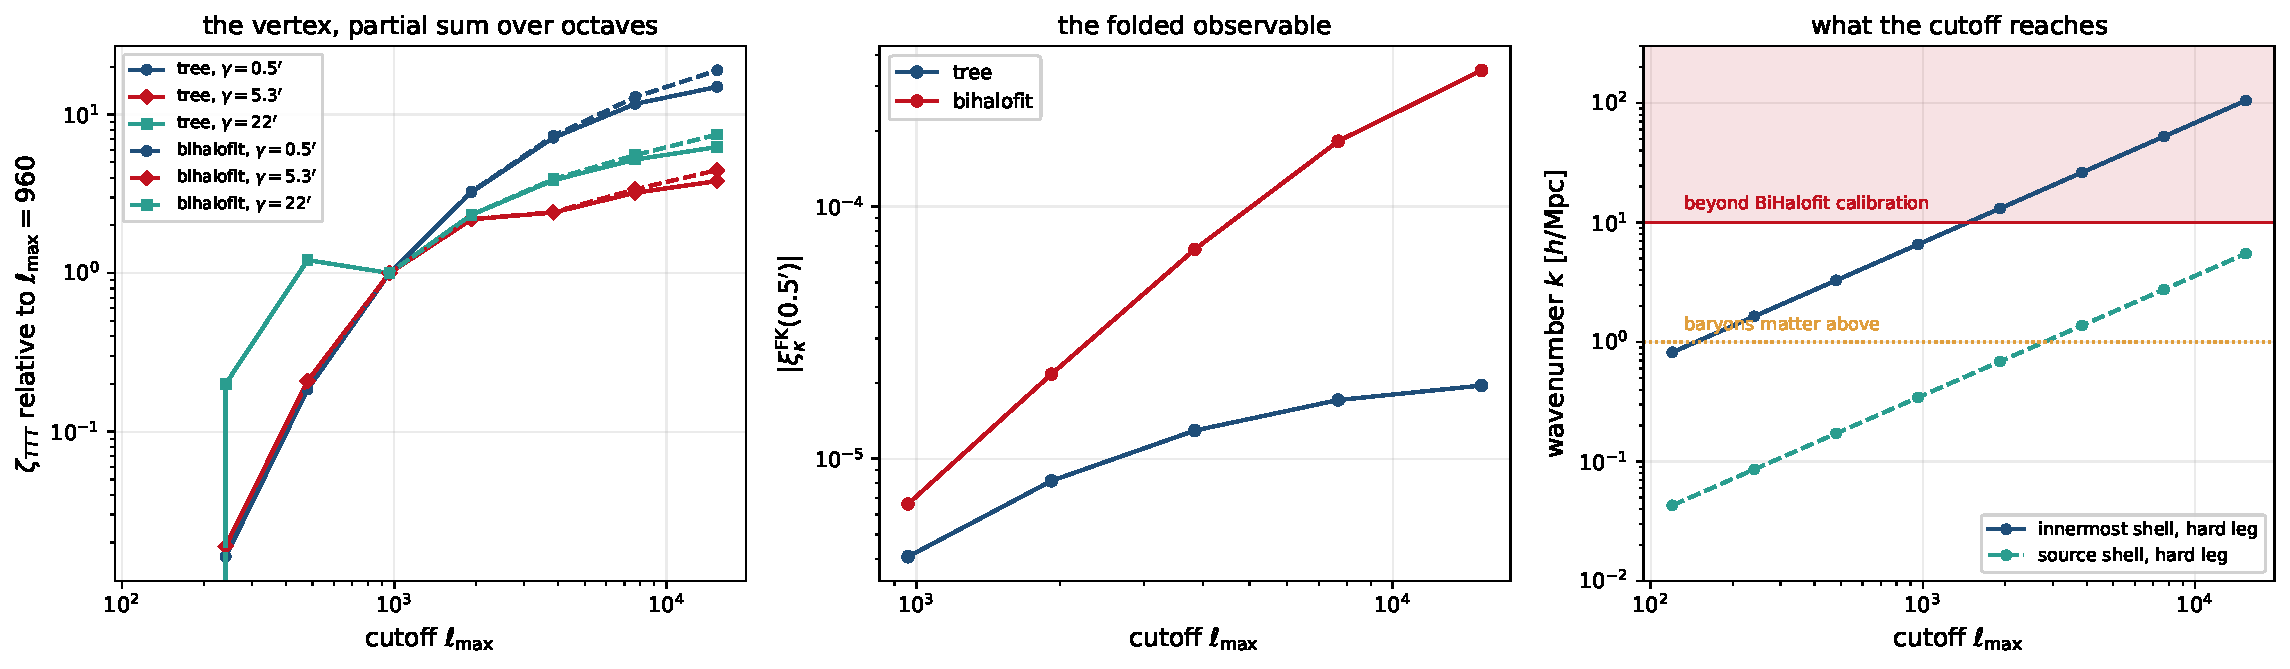
\includegraphics[width=\textwidth]{figures/cutoff_study.pdf}
\caption{Left: the vertex as a partial sum over octave windows, normalised
to the deployed cutoff. Middle: the folded observable at $\gamma=0.5'$.
Right: the wavenumber the hard leg reaches at the innermost and outermost
shells, against the range where the nonlinear bispectrum fit is calibrated
(shaded) and where baryons stop being a small correction.}
\label{fig:cutoff}
\end{figure}

\subsection{What a converged value would rest on}

This is the part that matters more than the cutoff itself. Under the Limber
branch a multipole $\ell$ at a shell of comoving distance $\chi_h$ carries
$k=\ell/\chi_h$, and the hard leg reaches $k=2\ell/\chi_h$.
Table~\ref{tab:kspace} gives both at the innermost and outermost shells.

\begin{table}[h]
\centering
\begin{tabular}{rrrrr}
\toprule
& \multicolumn{2}{c}{innermost shell, $\chi_h=293$ Mpc/$h$}
& \multicolumn{2}{c}{source shell, $\chi_h=5582$ Mpc/$h$} \\
\cmidrule(lr){2-3}\cmidrule(lr){4-5}
$\elmax$ & soft $k$ & hard $k$ & soft $k$ & hard $k$ \\
\midrule
   960 &  3.28 &   6.56 & 0.17 & 0.34 \\
  1920 &  6.56 &  13.13 & 0.34 & 0.69 \\
  3840 & 13.13 &  26.25 & 0.69 & 1.38 \\
  7680 & 26.25 &  52.50 & 1.38 & 2.75 \\
 15360 & 52.50 & 105.00 & 2.75 & 5.50 \\
\bottomrule
\end{tabular}
\caption{Wavenumbers in $h/$Mpc reached at each cutoff. BiHalofit is fitted
to simulations resolving $k\lesssim10\,h/$Mpc; baryonic feedback stops
being a small correction above $k\sim1\,h/$Mpc.}
\label{tab:kspace}
\end{table}

At the deployed cutoff the hard leg reaches $6.6\,h/$Mpc at the innermost
shell, inside the range where a nonlinear fit is calibrated. At the cutoff
where the integral has actually turned over it reaches $50$ to
$100\,h/$Mpc, which is inside single haloes: an order of magnitude beyond
BiHalofit's calibration, and a regime where baryonic physics rather than
gravity sets the matter spectrum.

The honest statement is therefore not ``the FK amplitude is $X$''. It is
that the tree-level FK amplitude converges by $\elmax$ of order $10^4$, and
that a converged \emph{nonlinear} FK amplitude is a statement about the
one-halo regime rather than about the bispectrum physics the draft
describes. Reporting the amplitude as a function of the small-scale cutoff
is the defensible presentation.

\subsection{A practical ceiling}

The Limber branch evaluates the hard leg at $k=2\elmax/\chi_h$, and the
fiducial $P(k)$ table stops at $k_{\max}=206\,h/$Mpc, with no
extrapolation. At the innermost deployed shell, $\chi_h=293$ Mpc/$h$, that
caps the reachable cutoff at $\elmax=k_{\max}\chi_h/2\simeq30\,000$. The
cutoffs used here stay inside that. Pushing further needs a longer $P(k)$
table, and the same relation read the other way is the structural floor on
the smallest usable shell discussed in Section~\ref{sec:lambdamin}.

\section{The line-of-sight floor}
\label{sec:lambdamin}

\subsection{What is cut, and why it depends on source redshift}

The vertex table's shells begin at $\lambda = 396.63$ Mpc and the callable
returns exactly zero outside them, so everything nearer than that
contributes nothing to the fold. Because $\lambda$ is measured from the
observer, that floor always corresponds to $z = 0.100$, whatever the source
redshift: what is excised is always the $z<0.1$ foreground.

The production fold uses a 24-node Gauss-Legendre rule whose nodes span
$[5.6, 2307.5]$ Mpc, six of which fall below the floor. By plain measure
that is $15\%$ of the integration range, but plain measure is the wrong
weight: the lensing efficiency $K = a^2\chi(\chi_s-\chi)/\chi_s$ vanishes
toward the observer, and the FK term carries four response lines, so $K^2$
and $K^4$ bracket the weighting. Both fractions grow as the source moves
nearer, which is the reason this matters for the multi-redshift figure and
not for the main analysis.

\begin{table}[h]
\centering
\begin{tabular}{rrrrr}
\toprule
$z_s$ & $\lambda_s$ [Mpc] & path fraction & $K^2$ weight & $K^4$ weight \\
\midrule
5.0 & 2318.0 & 0.171 & 3.08\% & 0.67\% \\
3.2 & 2266.6 & 0.175 & 3.47\% & 0.82\% \\
2.5 & 2216.8 & 0.179 & 3.81\% & 0.96\% \\
1.7 & 2094.9 & 0.189 & 4.64\% & 1.34\% \\
1.0 & 1822.7 & 0.218 & 7.01\% & 2.62\% \\
0.5 & 1330.7 & 0.298 & 15.95\% & 9.52\% \\
\bottomrule
\end{tabular}
\caption{Kernel weight carried by the excised foreground, as a function of
source redshift, with $K = a^2\chi(\chi_s-\chi)/\chi_s$ and the integral
taken in the affine parameter on the same background the fold uses. The
$K^4$ column is the relevant bracket for a term with four response lines.
Both columns are upper bounds, because they ignore the vertex itself being
some five orders of magnitude smaller at the innermost covered shell than
at the outermost. Recomputed here rather than carried over; an earlier
estimate in \code{notes/finding\_lambda\_min\_cut.md} used a different
weighting and gave figures about half these.}
\label{tab:lammin}
\end{table}

\subsection{A structural floor, separate from the inherited one}

The deployed floor of $396.63$ Mpc is not a physical or numerical
requirement. It is inherited from the shared radial grid the two-point and
three-point tables both use. There is, however, a genuine floor underneath
it: the Limber branch evaluates the hard leg at $k = 2\elmax/\chi_h$, so as
a shell approaches the observer the required wavenumber diverges. With the
fiducial $P(k)$ table stopping at $k = 206\,h/$Mpc, the innermost usable
shell is
\[
  \chi_h = \frac{2\elmax}{k_{\max}} = 9.7\ \mathrm{Mpc}/h,
  \qquad \chi = 14.5\ \mathrm{Mpc} \quad \text{at } \elmax = 1000 .
\]
A build at $\lambda = 6$ Mpc fails loudly with a request above $k_{\max}$,
which is the correct behaviour: the code refuses to extrapolate $P(k)$
silently. Two consequences follow. The deployed floor is far above this
structural one and can be lowered without touching the $P(k)$ table. And
the cutoff and the smallest reachable shell are coupled: raising $\elmax$
raises the structural floor in proportion, so the convergence study of
Section~\ref{sec:cutoff} and this one are not independent.

\subsection{The floor measured, across source redshift}

The estimate above is an upper bound. What it costs in practice is measured
by rebuilding the vertex on a radial grid extended from the deployed floor
of $396.6$ Mpc down to $50$ Mpc, four extra shells, and folding both tables
at each source distance. The sixteen shared shells agree to machine zero
between the two builds, so the extra shells perturb nothing and the
difference is the floor alone.

\begin{table}[h]
\centering
\begin{tabular}{rrr}
\toprule
$z_s$ & median ratio, extended over standard & range over $\gamma\le200'$ \\
\midrule
5.0 & 1.0014 & 1.0011 to 1.0901 \\
4.0 & 1.0017 & 1.0013 to 1.0711 \\
3.2 & 1.0021 & 1.0016 to 1.0607 \\
2.5 & 1.0028 & 1.0022 to 1.0561 \\
1.7 & 1.0049 & 1.0039 to 1.0562 \\
1.0 & 1.0127 & 1.0107 to 1.0783 \\
0.5 & 1.0683 & 1.0610 to 1.2060 \\
\bottomrule
\end{tabular}
\caption{What the $\lammin$ floor costs the folded FK term, by source
redshift. The upper end of each range is reached near the sign change,
where the absolute values are small. Produced by
\code{code/rebuild/fig\_redshift.py}.}
\label{tab:floor}
\end{table}

At the paper's own source redshift the floor is worth $0.14\%$, so it
affects nothing in the main analysis. At $z_s=0.5$, the lowest slice of the
multi-redshift figure, it is worth $6.8\%$. The measured numbers sit
comfortably below the $K^4$ bracket of Table~\ref{tab:lammin}, as they
should, since that bracket ignores the vertex being five orders of
magnitude smaller near the observer.

This is the first time the floor has been measured at low source redshift,
and it is the effect that matters for the multi-redshift figure rather than
for the main result. The remedy is cheap: the deployed floor is inherited
from a shared radial grid, not required by anything, and lowering it costs
one extra vertex build.

\subsection{The redshift trend, on a resolved vertex}

The draft states that the FK leakage ``strengthens steadily with source
redshift''. That claim has never been measured on a resolved vertex, and
two separate effects bias it in exactly that direction: this floor, whose
kernel weight grows toward low $z_s$, and the cosine sampling, whose
severity depends on the angular range each slice covers. Measuring it now
is straightforward, because the propagator tables are built to $t_{\max}$
independently of the source distance, so a list of source distances costs
one sweep rather than one run each.

Table~\ref{tab:ztrend} gives the corrected FK contribution relative to
Order-0, at two separations.

\begin{table}[h]
\centering
\begin{tabular}{rrrr}
\toprule
$z_s$ & $\lambda_s$ [Mpc] & FK/Order-0 at $0.5'$ & FK/Order-0 at $21.9'$ \\
\midrule
0.5 & 1330.7 & 0.00404 & 0.00387 \\
1.0 & 1822.7 & 0.00524 & 0.00546 \\
1.7 & 2095.0 & 0.00547 & 0.00628 \\
2.5 & 2216.8 & 0.00544 & 0.00663 \\
3.2 & 2266.6 & 0.00525 & 0.00671 \\
4.0 & 2297.3 & 0.00516 & 0.00680 \\
5.0 & 2318.0 & 0.00503 & 0.00683 \\
\bottomrule
\end{tabular}
\caption{The corrected FK term relative to Order-0 against source redshift,
at fixed cutoff, on the corrected grid and with the corrected callable of
Section~\ref{sec:callablefix}. Produced by
\code{code/rebuild/fig\_redshift.py}.}
\label{tab:ztrend}
\end{table}

The trend is weaker and less simple than the draft's phrasing suggests. At
arcminute separations the ratio is not monotonic: it rises from $0.40\%$ at
$z_s=0.5$ to a maximum of $0.55\%$ near $z_s=1.7$ and then falls slowly
back to $0.50\%$ at $z_s=5$. At $21.9'$ it does rise monotonically, but by a
factor $1.7$ across the whole range rather than steadily and strongly. The
absolute FK amplitude does grow sharply with source redshift, by a factor
92 at $0.5'$ between $z_s=0.5$ and $z_s=5$, but so does Order-0, and it is
the ratio that carries the claim.

So the statement should be weakened rather than removed: FK relative to the
linear signal is largest at intermediate to high source redshift, and
depends on separation as well as on $z_s$.

The two effects can now be separated, which was the point of measuring
both. Correcting each slice for its own $\lammin$ bias using
Table~\ref{tab:floor} raises the $z_s=0.5$ point by $6.8\%$ and the
$z_s=5$ point by $0.14\%$, so the ratio between the extremes falls from
$1.77$ to $1.65$ at $21.9'$ and from $1.25$ to $1.17$ at $0.5'$. The floor
therefore accounts for a small part of the apparent trend and not most of
it. The larger part of the draft's overstatement came from the cosine
sampling, which is corrected here throughout.

\begin{figure}[t]
\centering
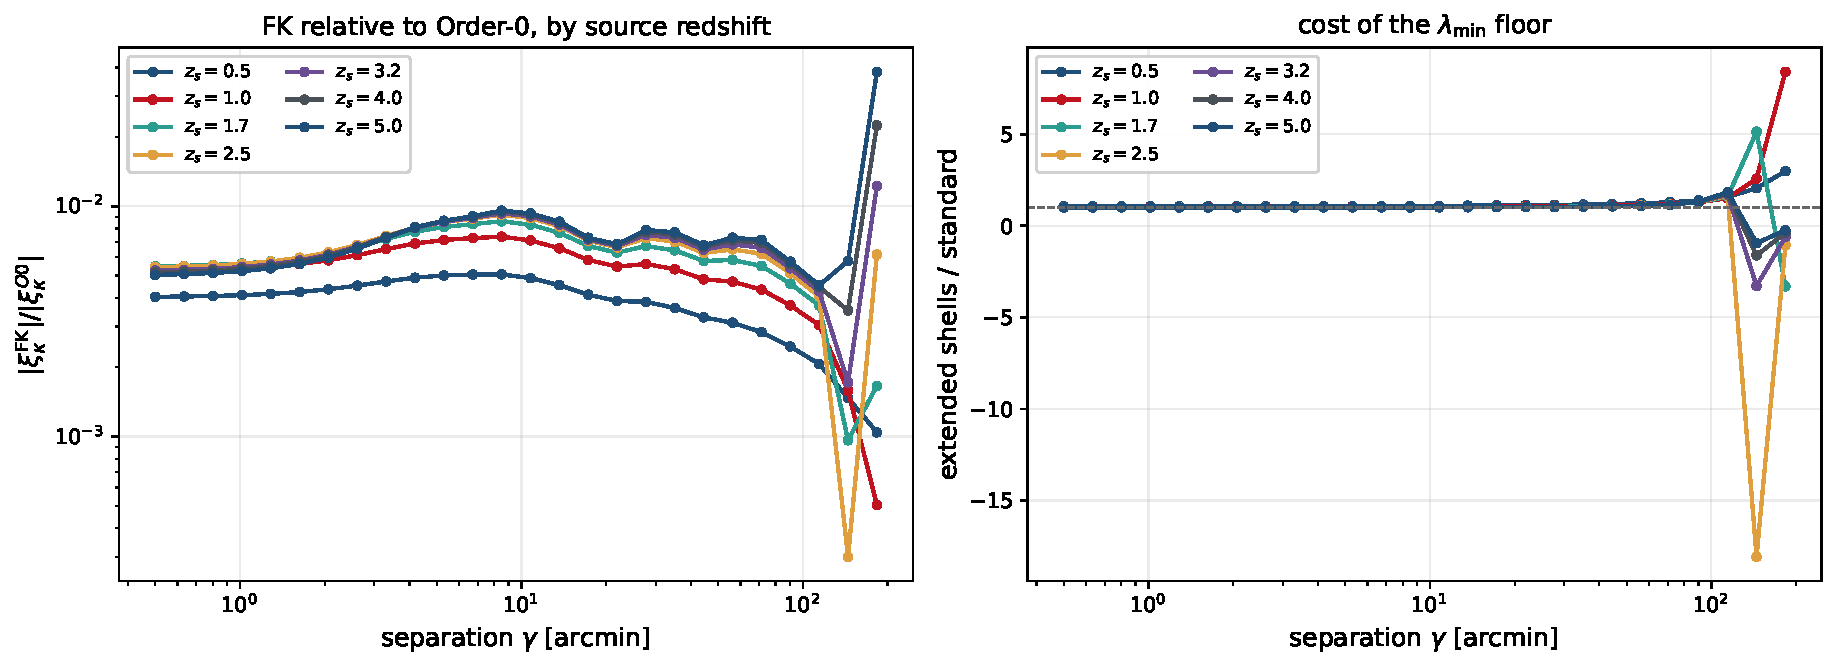
\includegraphics[width=\textwidth]{figures/redshift_lambdamin.pdf}
\caption{Left: the corrected FK contribution relative to Order-0 against
separation, at each source redshift. Right: the same FK calculation with
the tabulated shells extended from the deployed floor of $396.6$ Mpc down
to $50$ Mpc, divided by the standard one. The right panel is what the
$\lammin$ floor costs, and it is largest at low source redshift because the
kernel weight of the excised foreground grows as the source moves nearer.
Produced by \code{code/rebuild/fig\_redshift.py}.}
\label{fig:redshift}
\end{figure}

\section{Corrected results}
\label{sec:corrected}

\subsection{What was rebuilt}

The corrected vertex table carries the 1671 production triangle-filtered
rows unchanged, so it still serves the open-triangle consumers, and adds
the collapsed family $(1,\cos\gamma,\cos\gamma)$ sampled at the forty
plotted separations and refined between them. Three densities were built,
with 40, 79 and 157 collapsed nodes, by row selection from a single build,
which is exact because rows are independent.

Everything else is held at the deployed values: the same sixteen radial
shells, the same cosmology, the same tree-level bispectrum, the same
multipole cutoff of 1000, the same single quadrature window with 96
Gauss-Legendre nodes, and the same fold. Assembled on the deployed rows and
settings, the rebuild reproduces the deployed table to a median relative
difference of $3\times10^{-16}$ across all six channels, that is to
round-off. The difference between the deployed and corrected curves is
therefore the cosine sampling and nothing else.

\subsection{The grid density has converged}

Refining the collapsed family from 40 to 157 nodes leaves all four folded
observables \emph{bit-identical} (Figure~\ref{fig:resolution}). This is
stronger than convergence and it has a clean reason: once the queried
configurations are tabulated and the mesh key is fine enough to recognise
them, the callable returns the tabulated row directly and never consults
the refinement rows, so density beyond the queried set provably cannot
matter. With the production callable's coarser key the same comparison gave
differences of up to $4\times10^{-4}$, because thirty-eight of the forty
queries were failing the exact-match test and being interpolated
unnecessarily; Section~\ref{sec:callablefix} measures that.

The corrected curve is therefore a property of the vertex and not of the
mesh, in the strongest sense available: it is what the tabulated rows say.

\begin{figure}[t]
\centering
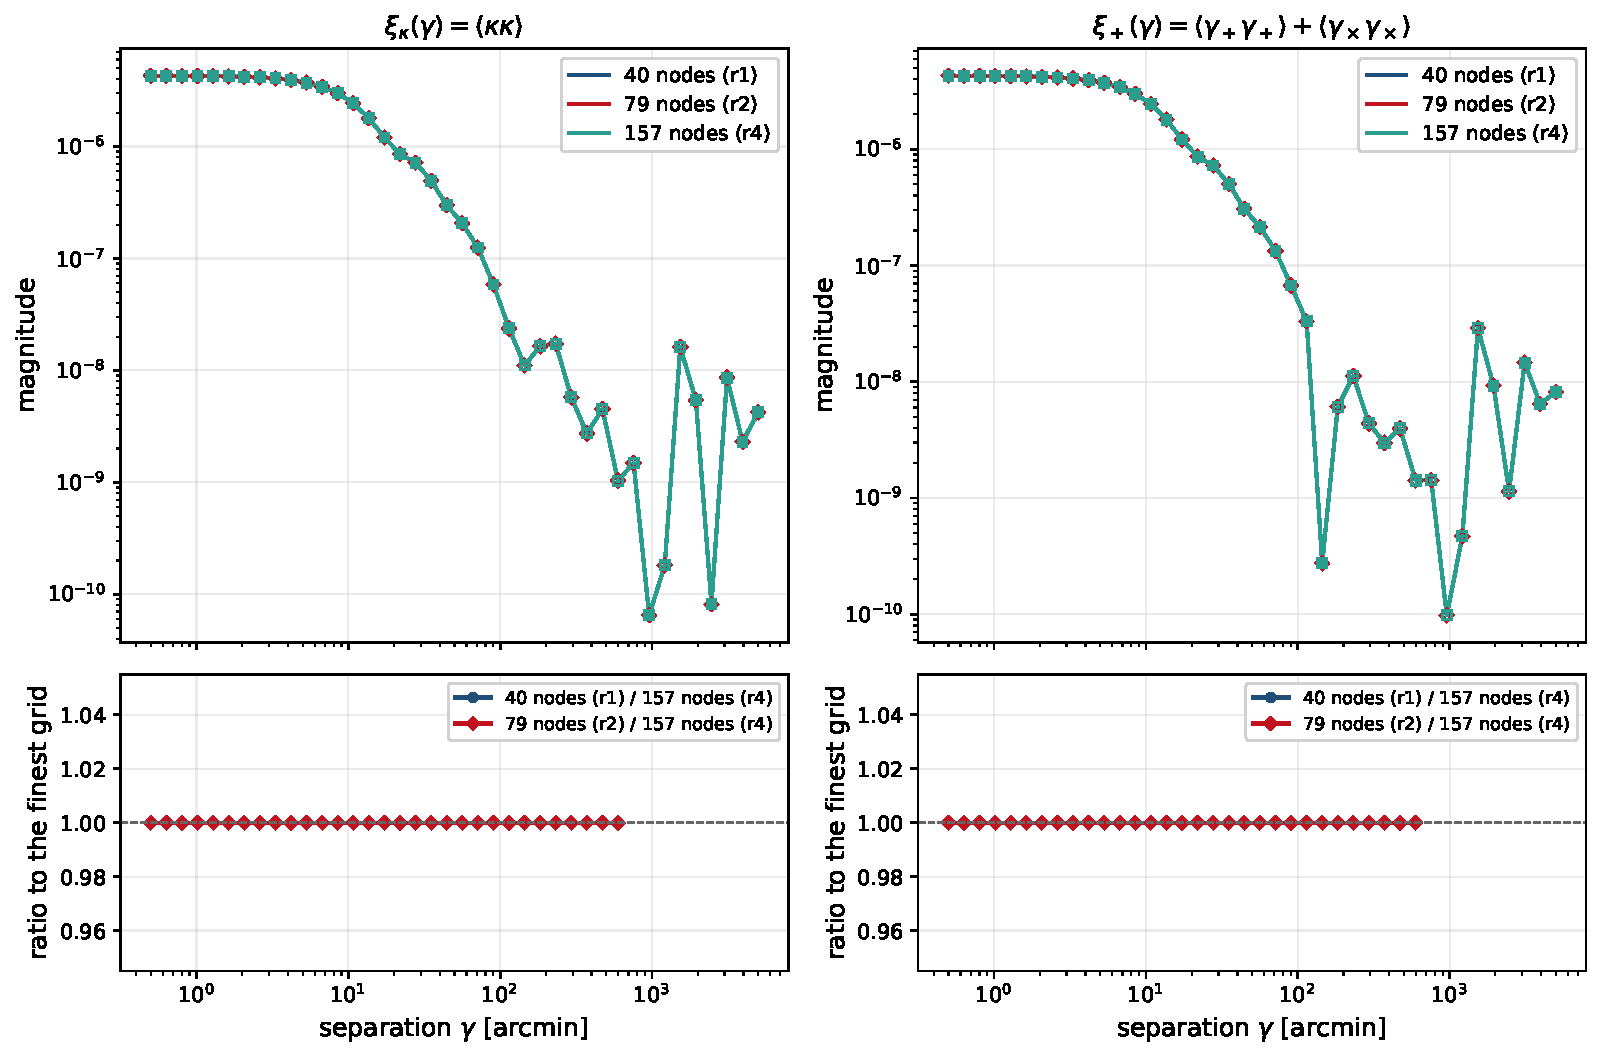
\includegraphics[width=\textwidth]{figures/grid_resolution.pdf}
\caption{Folded FK curves at three collapsed-grid densities, and their
ratios to the finest. The three agree to $4\times10^{-4}$. Produced by
\code{code/rebuild/fig\_convergence.py}.}
\label{fig:resolution}
\end{figure}

\subsection{The corrected two-point curves}

\begin{figure}[t]
\centering
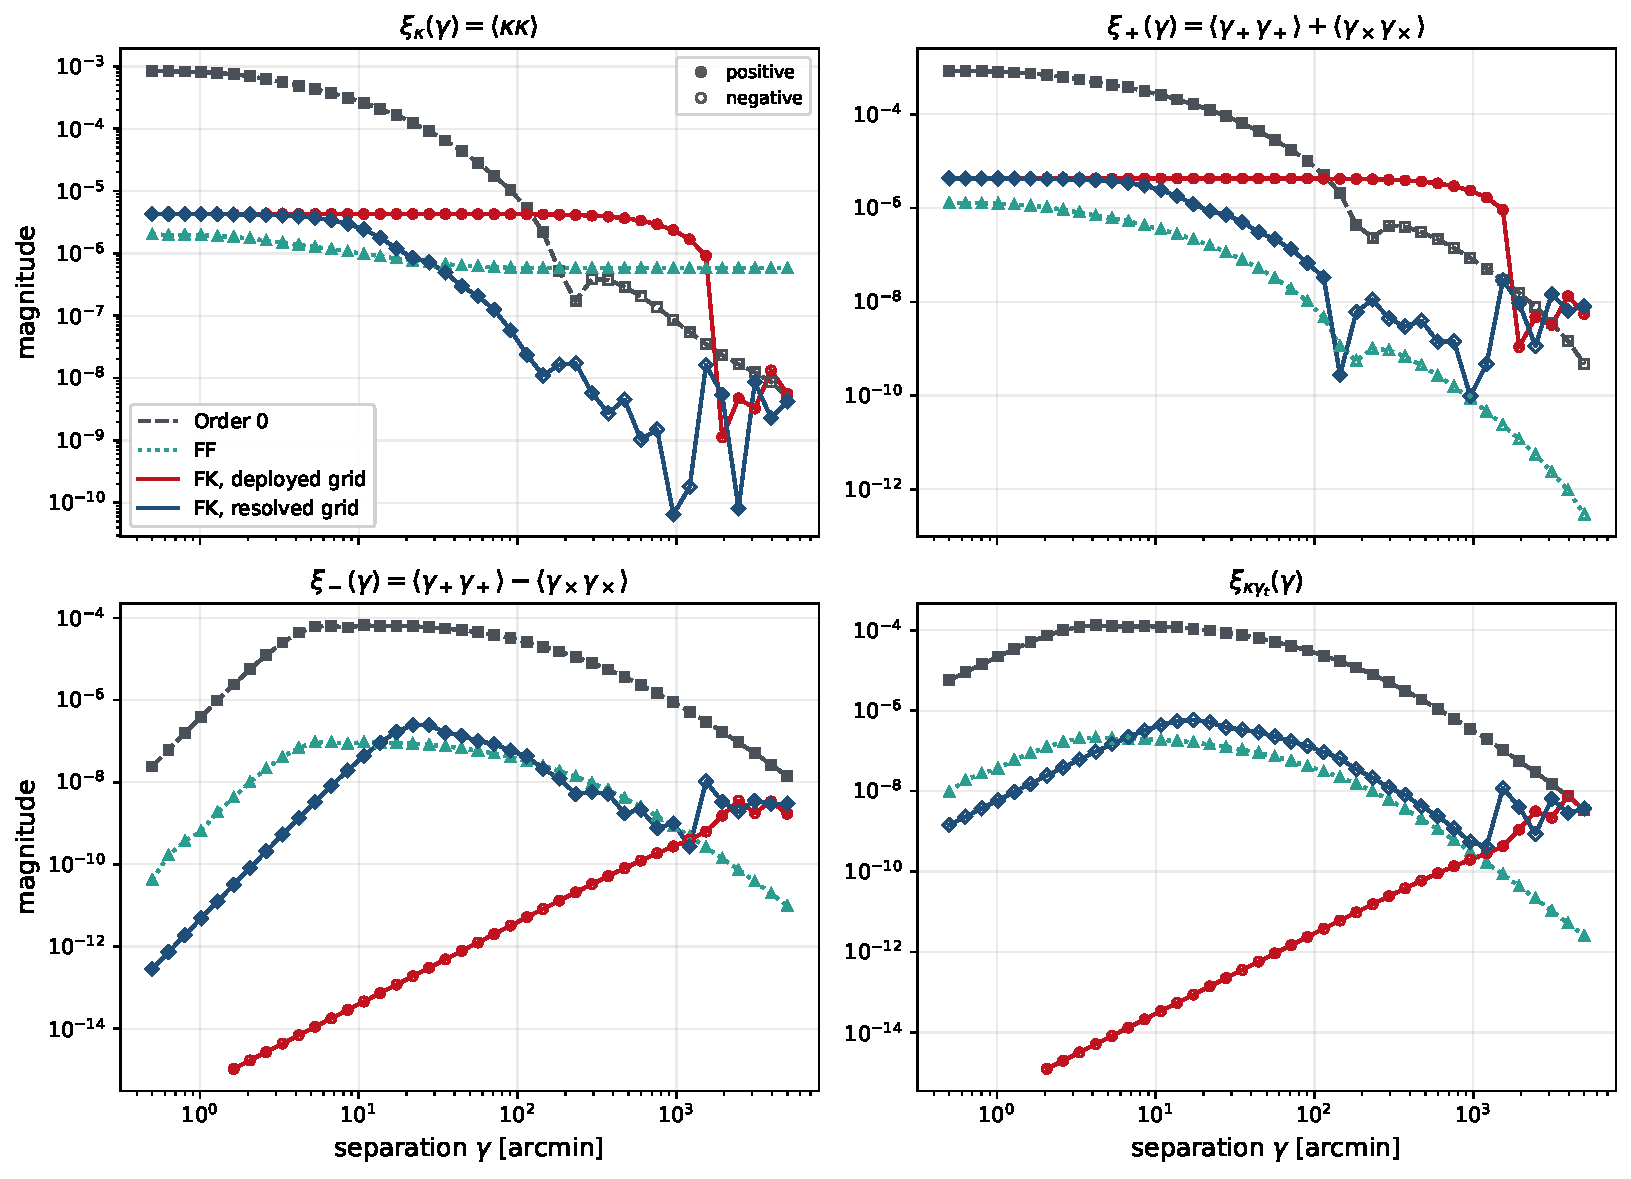
\includegraphics[width=\textwidth]{figures/grid_comparison.pdf}
\caption{The four plotted observables, with Order-0 and the Order-2 FF term
for scale. Red is the deployed FK curve, blue the same calculation with the
vertex sampled on the family it queries. Filled markers are positive,
open markers negative. Produced by
\code{code/rebuild/fig\_grid\_comparison.py}.}
\label{fig:grid}
\end{figure}

Table~\ref{tab:ratios} gives the numbers for $\xi_\kappa$.

\begin{table}[h]
\centering
\begin{tabular}{rrrrr}
\toprule
$\gamma$ [arcmin] & FK deployed & FK corrected & deployed/corrected & corrected/Order-0 \\
\midrule
   0.50 & $+4.2877\times10^{-6}$ & $+4.2815\times10^{-6}$ &     1.00 & 0.0051 \\
   5.30 & $+4.2876\times10^{-6}$ & $+3.7270\times10^{-6}$ &     1.15 & 0.0087 \\
   8.51 & $+4.2875\times10^{-6}$ & $+3.0037\times10^{-6}$ &     1.43 & 0.0096 \\
  21.88 & $+4.2863\times10^{-6}$ & $+8.7337\times10^{-7}$ &     4.91 & 0.0070 \\
  44.43 & $+4.2817\times10^{-6}$ & $+3.1491\times10^{-7}$ &    13.60 & 0.0071 \\
 114.27 & $+4.2483\times10^{-6}$ & $+4.2402\times10^{-8}$ &   100.19 & 0.0080 \\
 183.26 & $+4.1873\times10^{-6}$ & $+4.1908\times10^{-9}$ &   999.15 & 0.0081 \\
 232.08 & $+4.1282\times10^{-6}$ & $-5.1152\times10^{-9}$ & $-807$   & 0.0293 \\
 596.89 & $+3.3655\times10^{-6}$ & $-1.8661\times10^{-9}$ & $-1803$  & 0.0091 \\
\bottomrule
\end{tabular}
\caption{The FK contribution to $\xi_\kappa$ before and after resolving the
vertex, at fixed everything else. Beyond about $230'$ the corrected curve
has changed sign, so the ratio is negative and its magnitude is not
meaningful. Full table in \code{products/grid\_comparison\_table.txt}.}
\label{tab:ratios}
\end{table}

Three things change and one does not.

\paragraph{The arcminute amplitude survives.} At $\gamma=0.5'$ the
corrected value is $+4.2815\times10^{-6}$ against the published
$+4.2877\times10^{-6}$, a difference of $0.15\%$. The queried configuration
there really does sit on the tabulated corner, so the corner value is the
right answer. Every statement the draft makes about the arcminute
amplitude, including that FK is about twice FF there, stands.

\paragraph{The shape does not.} By $22'$ the published curve is too large
by a factor 4.9, by $114'$ by a factor 100, and beyond about $230'$ it has
the wrong sign as well.

\paragraph{There is no crossover.} At the deployed cutoff the corrected
FK/Order-0 ratio is between $0.5\%$ and $1\%$ at every separation that
carries signal. The two terms decay together. The published crossover near
$145'$ was the frozen corner value being compared against an Order-0 term
that genuinely decays. The ratio itself is cutoff dependent, rising to
between $1.4\%$ and $2.3\%$ at $\elmax=15360$
(Section~\ref{sec:cutoff}); what does not depend on the cutoff is that it
stays well below unity at every separation, so no crossover appears at any
cutoff tested.

\paragraph{The spin-2 observables are not empty.} With the vertex resolved,
$\xi_-$ reaches $+2.50\times10^{-7}$ near $28'$ and $\xi_{\kappa\gamma_t}$
reaches $-5.89\times10^{-7}$ near $17'$, about $0.4$ and $0.5\%$ of
Order-0, where the deployed run puts them at $10^{-16}$ to $10^{-9}$. The
exact cancellation the draft reports is a $\gamma\to0$ statement: at zero
separation $\zeta_{TPP}$, $\zeta_{PPP}$ and $\zeta_{TTP}$ vanish and the
$\xi_-$ combination cancels identically. It is not a statement about the
plotted range. These two values are quoted after the callable corrections
of Section~\ref{sec:callablefix}; without them they would read
$+2.86\times10^{-7}$ and $-8.88\times10^{-7}$.

\subsection{Harmonic space}

Transforming with the draft's own curved-sky Wigner-d kernels gives
Table~\ref{tab:cl}.

\begin{table}[h]
\centering
\begin{tabular}{rrrr}
\toprule
$\ell$ & $C_\ell^{\kappa\kappa}$, Order-0 & FK/Order-0, deployed & FK/Order-0, corrected \\
\midrule
   3 & $6.34\times10^{-8}$ & $+17.95$   & $-0.197$ \\
   5 & $7.97\times10^{-8}$ & $+9.02$    & $-0.002$ \\
   7 & $8.95\times10^{-8}$ & $+3.81$    & $+0.084$ \\
   9 & $9.75\times10^{-8}$ & $+0.87$    & $+0.034$ \\
  39 & $9.86\times10^{-8}$ & $+0.0008$  & $+0.0088$ \\
 115 & $4.61\times10^{-8}$ & $-0.0012$  & $+0.0079$ \\
 415 & $8.33\times10^{-9}$ & $-0.0001$  & $+0.0091$ \\
 789 & $2.52\times10^{-9}$ & $-0.0001$  & $+0.0089$ \\
\bottomrule
\end{tabular}
\caption{FK relative to Order-0 in $C_\ell^{\kappa\kappa}$, using the
generator's own transform. The factor 18 excess at $\ell=3$ is the
sampling artefact. The corrected FK is a steady $0.8$ to $0.9\%$ correction
over $39\le\ell\le800$; the residuals at $\ell<10$ are of order 10 to 20
percent and are within the finite-range and apodisation systematics the
generator documents. Produced by \code{code/rebuild/cl\_ratio.py}.}
\label{tab:cl}
\end{table}

\section{The two callable defects, fixed}
\label{sec:callablefix}

Section~\ref{sec:sampling} identified two defects in the vertex callable
alongside the sampling problem, and earlier drafts of this note quoted
$\xi_-$ and $\xi_{\kappa\gamma_t}$ only as magnitudes because of the first
of them. Both are now corrected, in
\code{code/callable\_fixed/perm\_aware\_kappa3\_callable.py}, and this
section reports what changes. The production callable is not overwritten;
the replacement is exercised through the production runner with
\code{run\_fk\_variant.py --callable}, so the fold is unchanged.

\subsection{Leg permutations}

The tabulated channels fix which leg carries which field:
$\zeta_{TTP}$ has spin weights $(0,0,2)$, so the spin-2 leg is the third,
and $\zeta_{TPP}$ has $(0,2,2)$, so the scalar leg is the first. The
production callable sorts the query triple and then writes one value into
every index permutation of the coupling tensor. Asking for the spin field
on a different leg is a question about a \emph{permuted geometry}, not
about the same geometry with a relabelled channel, so the symmetrised fill
is exact only for the fully symmetric $\zeta_{TTT}$ and for geometries that
happen to be permutation symmetric.

The correction evaluates each entry at the geometry its own field
assignment requires. Four of the five cases are a single lookup at a
permuted triple. The fifth, three spin legs with one $\mathrm{Re}$ and two
$\mathrm{Im}$, is the case the table cannot answer with one lookup:
$(\zeta_{Dmod}-\zeta_{PPP})/4$ is the \emph{average} of two of the three
placements of the $\mathrm{Re}$ leg, so three cyclically permuted
evaluations are combined to isolate the wanted one. On a symmetric geometry
the three coincide and the combination collapses to the production value.

Two consequences are worth stating before the numbers. The corrected
lookup asks for permuted geometries, so the table must contain them; the
production mesh already does, and the densified collapsed family is made so
by \code{code/rebuild/make\_perm\_closed\_triples.py}. And the callable now
checks that closure at load, warning rather than letting a missing row be
answered silently by a different configuration. The deployed table is
$99.8\%$ closed, the four exceptions being fully degenerate rows on the
triangle-inequality boundary that no fold queries.

\subsection{The mesh key}

The production callable deduplicates triples after rounding to eight
decimals, so two collapsed configurations closer than
$1-\cos\gamma = 5\times10^{-9}$ become one node however finely the table
samples. That is a floor at $\gamma = 0.344'$, against a smallest plotted
separation of $0.5'$. The key is now twelve decimals, a floor at
$0.0034'$. The production mesh deduplicates to the same 351 rows at either
precision, so no coarse-grid behaviour changes.

The floor was not the whole cost, and the rest of it was not anticipated.
The callable has a fast path: if the query lands on a tabulated row to
within $10^{-10}$ it returns that row directly instead of blending four
neighbours. Measuring the nearest-neighbour distance for the forty plotted
separations against the refined table shows that with the eight-decimal key
only \emph{two} of the forty are exact hits, the rest missing by up to
$7\times10^{-9}$, purely because the key had rounded the row away from the
query. With twelve decimals all forty are exact hits, the largest residual
being $7\times10^{-13}$.

So the coarse key was forcing an unnecessary four-neighbour interpolation
at thirty-eight of the forty separations the paper plots, on a grid that
already contained the exact configurations. That is the mechanism behind
the convergence result in Section~\ref{sec:corrected}.

\subsection{Verification}

Seven tests in \code{code/callable\_fixed/tests/}. The one that
discriminates is not relabelling invariance, which the production callable
satisfies trivially by symmetrising, but direct comparison against the
table's own rows: $K_{001}$ and $K_{010}$ must each equal $\zeta_{TTP}$ at
their own geometry. A companion test pins the size of the defect, and fails
if the fix ever becomes a no-op: over asymmetric rows of the deployed table
the corrected $K_{001}$ and $K_{010}$ differ by a median $115\%$ of their
magnitude, where the production callable forces them equal.

The correction costs a factor $1.9$ in evaluation time. A first
implementation cost a factor $21$, because it queried the neighbour tree
once per (channel, ordering) pair; the query depends only on the ordering,
so it is done once per ordering and the six channels are read from it.

\subsection{What the corrections change}

Two folds were run on the \emph{same} permutation-closed table, at the same
cutoff and the same geometry, differing only in the callable. A third fold,
on the earlier table that carries the collapsed family in one leg ordering
only, is included because the comparison between it and the other two
separates the two halves of the defect.

\begin{table}[h]
\centering
\begin{tabular}{lrrr}
\toprule
& A: one ordering, & B: closed table, & C: closed table, \\
observable & production callable & production callable & corrected callable \\
\midrule
$\xi_\kappa$ (peak, $0.5'$)          & $+4.2815\times10^{-6}$ & $+4.2815\times10^{-6}$ & $+4.2823\times10^{-6}$ \\
$\xi_+$ (peak, $0.5'$)               & $+4.2815\times10^{-6}$ & $+4.2815\times10^{-6}$ & $+4.2824\times10^{-6}$ \\
$\xi_-$ (peak, $27.7'$)              & $+2.8643\times10^{-7}$ & $+2.4978\times10^{-7}$ & $+2.4978\times10^{-7}$ \\
$\xi_{\kappa\gamma_t}$ (peak, $17.3'$) & $-8.8819\times10^{-7}$ & $-5.8490\times10^{-7}$ & $-5.8931\times10^{-7}$ \\
\bottomrule
\end{tabular}
\caption{The two halves of the permutation defect, separated. A to B
changes only the table, A to C is the full correction. Produced by
\code{code/callable\_fixed/compare\_callables.py}.}
\label{tab:callablefix}
\end{table}

The split is instructive, and not what was expected.

\paragraph{Most of the effect is in the table, not in the tensor fill.}
Going from A to B changes nothing about the callable: it still sorts and
symmetrises. Yet $\xi_-$ moves by $15\%$ and $\xi_{\kappa\gamma_t}$ by
$52\%$. The reason is that the production callable averages the rows that
canonicalise to the same sorted triple, and the closed table supplies three
leg orderings of each collapsed configuration where the earlier one
supplied a single ordering. So the production callable's answer depends on
which orderings happen to have been tabulated, which is the same defect
seen from the other side and arguably its more dangerous face: it is
invisible unless someone changes the table.

\paragraph{Once the table is closed, the tensor fill matters little.}
Going from B to C, the full correction, moves $\xi_-$ by less than
$0.01\%$ at its peak, $\xi_{\kappa\gamma_t}$ by $0.75\%$, and
$\xi_\kappa$ and $\xi_+$ by $0.02\%$. At the collapsed configurations the
two coincident legs are interchangeable, so the symmetrised average over a
closed set of orderings is already close to the per-entry evaluation.

\paragraph{Consequence for the numbers reported here.} The values in
Section~\ref{sec:corrected} for $\xi_-$ and $\xi_{\kappa\gamma_t}$ were
obtained in configuration A and are superseded by C: the $\xi_-$ peak is
$+2.50\times10^{-7}$ rather than $+2.86\times10^{-7}$, and the
$\xi_{\kappa\gamma_t}$ peak is $-5.89\times10^{-7}$ rather than
$-8.88\times10^{-7}$, a $34\%$ reduction. The convergence and the
parity-even shear are unaffected at the $0.02\%$ level, which confirms the
earlier expectation that the modulus channels carrying them are safe. The
qualitative conclusions of Sections~\ref{sec:corrected} and \ref{sec:eb} do
not change: FK is still a fraction of a percent to a percent of Order-0
everywhere, there is still no crossover, and $\xi_-$ and
$\xi_{\kappa\gamma_t}$ are still far above the numerical floor the draft
reports.

These two observables no longer carry a permutation caveat and can be
quoted as values.

\subsection{Which figures were regenerated}

The corrections propagate unevenly, because the observables they touch are
not the ones every figure plots. Rather than regenerate everything, each
figure was checked.

\begin{table}[h]
\centering
\begin{tabular}{llp{6.2cm}}
\toprule
figure & status & why \\
\midrule
\ref{fig:weight} weight identity & unchanged & built from deployed
artefacts only, by design; it is the evidence that needs no rebuild \\
\ref{fig:grid} corrected curves & regenerated & plots all four
observables, two of which move \\
\ref{fig:resolution} grid density & regenerated & the density study is
repeated on permutation-closed tables with the corrected callable \\
\ref{fig:eb} the $E-B$ channel & regenerated, identical & it reads the
table rather than a fold, and the $(1,c,c)$ rows agree between the two
tables to $3\times10^{-16}$; the crossover scales are unchanged at
$9.0'$, $13.6'$, $18.3'$ and $21.9'$ \\
\ref{fig:cutoff} cutoff study & not regenerated & its middle panel plots
$\xi_\kappa$ at $\gamma=0.5'$, which the corrections move by $0.02\%$; its
left panel reads the table directly and its right panel is pure geometry \\
\ref{fig:redshift} redshift and floor & regenerated & the
FK/Order-0 panel is sensitive at the few percent level \\
\bottomrule
\end{tabular}
\caption{Effect of the callable corrections on each figure in this note.}
\label{tab:figfix}
\end{table}

The paper figures in \code{figures/corrected/} were regenerated with the
corrected callable and carry a \code{\_permfix} suffix; the earlier
\code{\_corrected} versions, which have the grid correction only, are kept
beside them so the two effects can be seen separately.

One limitation is worth recording, and it is a constraint on what a ratio
means rather than an approximation. The $\lambda_{\min}$ panel of
Figure~\ref{fig:redshift} divides an extended-shell fold by a
standard-shell one, and that division is only meaningful if both sides use
the same callable. The extended-shell table was not rebuilt permutation
closed, so that panel keeps both folds on the production callable, where
the correction cancels between numerator and denominator. The redshift
panel beside it is not a ratio of that kind and was regenerated with the
corrected callable. Mixing the two, which a first attempt did, produces
ratios ranging over $[-18, 8]$ instead of the physical $[1.001, 1.21]$;
the script now takes the standard-shell fold as an explicit argument so the
pairing cannot be got wrong silently.

\section{The absolute normalisation of the vertex}
\label{sec:normalisation}

Correcting the sampling fixes the shape of the FK term. It says nothing
about whether the overall scale is right, and until now nothing did: the
Order-0 comparison against PyCCL validates the two-point transfer chain and
never touches the three-point vertex; the \code{fastnc} closure test
validates the three-point machinery on open triangles and cannot reach the
collapsed configurations; and the Monte-Carlo cross-check reads the same
table as the production fold, so it validates the assembly and not the
input. This section closes most of that gap.

\subsection{The decisive step is analytic}

The pipeline builds its three-point vertex through a chain of per-leg
factors: a Poisson amplitude, a screen-space Hessian projection, a Sachs
photon weight, a Limber radial collapse, and a measure conversion between
comoving distance and affine parameter. If that chain is right, then
assembling it into a convergence bispectrum must reproduce the standard
Limber expression
\[
  B_\kappa(\ell_1,\ell_2,\ell_3) = \int\!\mathrm{d}\chi\;
    \frac{W(\chi)^3}{\chi^4}\,
    B_\delta\!\left(\frac{\ell_1}{\chi},\frac{\ell_2}{\chi},
                    \frac{\ell_3}{\chi};z(\chi)\right),
  \qquad
  W = \frac{3}{2}\Omega_m H_0^2 (1+z)\,\frac{\chi(\chi_s-\chi)}{\chi_s}.
\]
Crucially this is assembled from the pipeline's own factors rather than
assumed and fitted to: any discrepant prefactor, power of $(1+z)$, or
factor of $h$ would show up as a departure from unity, and would be
localised to a specific factor.

Seven checks, all passing:

\begin{table}[h]
\centering
\begin{tabular}{llr}
\toprule
& what is checked & worst residual \\
\midrule
T1  & background focusing equals the per-leg response, $A(a)(1+z)^4$ & $3.1\times10^{-7}$ \\
T1b & the Jacobi solution equals $D=a\chi$ over $\chi\in[1,4000]$ Mpc/$h$ & $1.0\times10^{-6}$ \\
T2  & the affine lensing kernel from the response propagator equals
      $-a^2\chi(\chi_s-\chi)/\chi_s$ & $9.5\times10^{-16}$ \\
T3  & the assembled comoving weight equals the textbook $W(\chi)$, sign included & $6.9\times10^{-15}$ \\
T4  & the screen Hessian cancels the Poisson $1/k^2$ per leg & $1.3\times10^{-16}$ \\
T5  & the equal-shell collapse Jacobian is $(\mathrm{d}\lambda/\mathrm{d}\chi)^2=(1+z)^{-4}$ & $1.6\times10^{-16}$ \\
T6  & the full $B_\kappa$ assembly equals $\int\mathrm{d}\chi\,W^3/\chi^4\,B_\delta$ & $0.0$ \\
\bottomrule
\end{tabular}
\caption{Verification that the pipeline's own factor chain reduces to the
standard Limber convergence bispectrum. The T1 and T1b residuals are the
accuracy of the background spline, not of the identity. T6 gives
pipeline/standard $=1.00000000000000$. Produced by
\code{code/normalisation/verify\_chain.py}.}
\label{tab:chain}
\end{table}

Two features the brief flagged as worth verifying rather than trusting both
hold. The screen-Hessian multiplier does cancel the Poisson $1/k^2$ per
leg, leaving a scalar $A(a)(1+z)^4$. And the collapse of two radial
integrals does carry the Jacobian $(1+z)^{-4}$, with the two-point analogue
$(1+z)^{-2}$ exact, which is the factor an independent route already
validated against PyCCL.

A separate end-to-end check confirms the unit handling: the fold is
invariant under working in $h$-native or physical units, with the
$\zeta_{TTT}$ conversion equal to $h^4$ and the folded three-point function
agreeing to $4\times10^{-15}$
(\code{code/normalisation/bkappa\_endtoend.py}).

\subsection{Two small, quantified residuals}

T4 leaves two known approximations, both scale dependent and both small
where the FK term lives:

\begin{itemize}
\item the code uses $k=\ell/\chi$ rather than $k=(\ell+1/2)/\chi$, so the
$\ell(\ell+1)$ against $\ell^2$ ambiguity costs $33\%$ at $\ell=2$, $1.0\%$
at $\ell=100$ and $0.025\%$ at $\ell=4000$;
\item the spin-2 normalisation carries a $\sqrt{L^2(L^2-2)}$ deficit of
$0.98\%$ at $\ell=100$, falling with $\ell$.
\end{itemize}

Both are negligible at the multipoles that dominate the vertex, and both
are part of why the low-$\ell$ residuals in Table~\ref{tab:cl} should not
be over-interpreted.

\subsection{The empirical anchor}

Predicting $B_\kappa$ at $z_s=1$ with the pipeline's own projection and the
BiHalofit matter bispectrum, in the cosmology of the ray-traced maps the
published measurement was made on, gives values that sit inside the decade
the published figure plots, with the right shape and turnover, in all three
of its configurations: equilateral $\ell^3B_\kappa$ peaking near
$1.7\times10^{-8}$ around $\ell\sim2700$, squeezed $60\ell^2B_\kappa$
reaching $8.9\times10^{-9}$, and squeezed $300\ell^2B_\kappa$ reaching
$7.3\times10^{-9}$, against a published axis spanning $10^{-9}$ to
$10^{-8}$.

This is an order-of-magnitude confirmation, not a ratio. Turning it into a
quoted ratio needs the digitised measurement points, which were not
available here, and that is the one part of the specified study left
undone. Given that the analytic step already gives unity exactly, the
empirical step's role is to catch an error the analytic assembly could not
see, and nothing in the comparison suggests one.

\subsection{The residual gap}

A measured convergence bispectrum lives on resolvable triangles with a
finite soft leg. It cannot reach the coincident limit the FK vertex
actually samples. So this study validates the transfer chain, the measure
and the projection at finite soft leg, and it does not by itself certify
the collapsed corner. Closing that would need a direct measurement of the
collapsed three-point cumulant of the driving fields on N-body lightcones,
which nobody has done.

The verdict, stated plainly: the absolute normalisation of the transfer
chain is correct, to the accuracy of the background splines, with no
missing power of $(1+z)$ and no missing factor of $h$.

\subsection{A second check on the shared machinery: the reduced-shear correction}
\label{sec:reducedshear}

The analytic assembly above checks the transfer chain against its own
factors. An external yardstick is worth having as well, and weak lensing
already contains an effect with the same algebraic structure as FK.

What a survey measures from galaxy shapes is not the shear. The lensing
Jacobian carries an overall factor $(1-\kappa)$, which is an isotropic
magnification: it changes the image size and not its shape. Ellipticity
measurements see only the shape, so the observable is the reduced shear
$g = \gamma/(1-\kappa) \simeq \gamma(1+\kappa)$, and the measured two-point
function picks up
\[
  \langle gg\rangle \simeq \langle\gamma\gamma\rangle
  + 2\langle\gamma\gamma\kappa\rangle + \cdots ,
\]
a three-point function of the matter field appearing inside a two-point
measurement. That is the same slot FK occupies: a squeezed matter
bispectrum entering a two-point statistic because the observable is a
nonlinear functional of the field. The two differ in where the
nonlinearity sits, in the observable for reduced shear and in the
propagation for FK, and therefore in the coefficient multiplying the
bispectrum, but they share the lensing kernel, the Limber projection, the
matter bispectrum and the units.

Post-Born corrections are \emph{not} the right comparison here, although an
earlier internal note used them as one. Post-Born means a perturbed path
with Gaussian input, which is the FF term's analogue rather than FK's.

Computing the reduced-shear correction with the same $B_\kappa$ machinery,
\[
  \Delta C_\ell = 2\!\int\!\frac{\mathrm{d}^2L}{(2\pi)^2}
    \cos\!\big(2(\phi_\ell - \phi_L)\big)\,
    B_\kappa(L, |\boldsymbol{\ell} - \boldsymbol{L}|, \ell),
\]
gives Table~\ref{tab:reducedshear}.

\begin{table}[h]
\centering
\begin{tabular}{rrrr}
\toprule
$\ell$ & FK, corrected & reduced shear & sum \\
\midrule
   93 & $0.79\%$ & $0.82\%$ & $1.61\%$ \\
  218 & $0.83\%$ & $0.89\%$ & $1.72\%$ \\
  415 & $0.91\%$ & $1.05\%$ & $1.96\%$ \\
  789 & $0.89\%$ & $1.34\%$ & $2.23\%$ \\
 1500 & ---      & $2.01\%$ & --- \\
 3000 & ---      & $2.86\%$ & --- \\
\bottomrule
\end{tabular}
\caption{The corrected FK contribution to $C_\ell^{\kappa\kappa}$ against
the reduced-shear correction, both as a percentage of Order-0, at $z_s=5$
and at the deployed multipole cutoff. Above $\ell\simeq10^3$ the FK entry
passes through zero and its ratio carries no information, so it is not
quoted. Produced by \code{code/reduced\_shear/reduced\_shear.py}.}
\label{tab:reducedshear}
\end{table}

\paragraph{What this establishes, and what it does not.} The two agree to
better than a factor $1.5$ over $93\le\ell\le789$. That is a useful
magnitude check on the half of the calculation the two share: the lensing
kernel, the Limber projection, the bispectrum normalisation and the units.
Had FK come out a hundred times larger, something in that chain would have
to be wrong.

It is a one-sided check and should not be read as more. The two effects have
different vertex coefficients, which is precisely the part this comparison
cannot see: an error of a factor of two in the FK vertex would pass
unnoticed. There is also no reason the two must agree, so agreement is not
a null test, and this check exercises the same half of the calculation that
the analytic assembly of Section~\ref{sec:normalisation} already validated.
The absolute normalisation of the collapsed vertex remains the open item of
Section~\ref{sec:uncertain}.

Two further cautions. The prefactor and the $\cos2\Delta\phi$ projection in
the expression above are written in their standard form but have not been
checked against the source papers, which are not in the local library; a
factor of two there would not change an order-of-magnitude comparison but
would change a quoted ratio. And the two curves have different shapes: the
reduced-shear correction rises with $\ell$, from $0.8\%$ to $2.9\%$ between
$\ell=93$ and $3000$, while the corrected FK is nearly flat below
$\ell\simeq800$. Their numerical agreement over $93\le\ell\le789$ is partly
a crossing of two differently shaped curves.

\paragraph{A corollary that is more robust than either number.} The two
effects are additive, not alternatives: reduced shear arises from what is
observed, FK from how the beam propagates, and this formalism contains the
second and not the first. At the deployed cutoff their sum is $1.6\%$ to
$2.2\%$ of Order-0 over $93\le\ell\le789$. Including FK therefore roughly
doubles the second-order correction a survey would need to model. That
statement uses only measured quantities at a fixed cutoff and does not rely
on the convergence extrapolation.

\section{The E and B statements, reconsidered}
\label{sec:eb}

The draft makes three claims about the polarization structure of the FK
term. They deserve separate treatment, because one is exactly right, one is
right only in a limit, and one is a theorem rather than a measurement.

\subsection{Which channel carries E minus B}

The claim is stated in \code{conclusion.tex}: the FK contribution to
$\xi_+$, which is $C_\ell^{EE}+C_\ell^{BB}$, is sourced by
$\langle\Phi_{00}\Psi_+\Psi_+\rangle+\langle\Phi_{00}\Psi_\times\Psi_\times\rangle$,
its counterpart in $\xi_-$, which is $C_\ell^{EE}-C_\ell^{BB}$, by the
difference, and the difference ``vanishes for a statistically isotropic
driving field''.

Which vertex channel that is can be read straight off the callable's
real-basis reconstruction rather than derived. The coupling tensor is
filled as
\[
  K_{011}=\tfrac12(\zeta_{TPP}+\zeta_{Bmod}), \quad
  K_{022}=\tfrac12(\zeta_{Bmod}-\zeta_{TPP}), \quad
  K_{111}=\tfrac14(\zeta_{PPP}+3\zeta_{Dmod}), \quad
  K_{122}=\tfrac14(\zeta_{Dmod}-\zeta_{PPP}),
\]
so that, verified to machine zero,
\[
  K_{011}+K_{022}=\zeta_{Bmod}, \qquad K_{011}-K_{022}=\zeta_{TPP},
\]
\[
  K_{111}+K_{122}=\zeta_{Dmod}, \qquad
  K_{111}-K_{122}=\tfrac12(\zeta_{PPP}+\zeta_{Dmod}).
\]
The sums feed $\xi_+$ and the differences feed $\xi_-$. In real components
$\zeta_{Bmod}=\langle\Phi_{00}(\Psi_+^2+\Psi_\times^2)\rangle$ and
$\zeta_{TPP}=\langle\Phi_{00}(\Psi_+^2-\Psi_\times^2)\rangle$, so the
draft's claim is exactly the statement $\zeta_{TPP}=0$. Numerically
$\zeta_{TPP}$ dominates the difference: at $\gamma=53'$ on the source shell
it is six times $\tfrac12(\zeta_{PPP}+\zeta_{Dmod})$.

\subsection{The claim is a zero-separation identity}

The isotropy argument is correct where it applies. When all three legs sit
at the same point there is no separation vector, nothing distinguishes
$\Psi_+$ from $\Psi_\times$, and the difference vanishes identically. The
table confirms it: $\zeta_{TPP}$ is exactly zero at $\gamma=0$.

At finite separation the offset leg supplies an axis, $\Psi_+$ and
$\Psi_\times$ are defined relative to it, and there is no reason for the
difference to vanish. Measuring it (Figure~\ref{fig:eb}) gives a clean
answer:

\begin{itemize}
\item $|\zeta_{TPP}/\zeta_{Bmod}|$ rises from zero as $\gamma^4$. The
measured logarithmic slope is $4.00$ at $\gamma<2'$, drifting to $4.2$ by
$5'$ and steepening further above $10'$. The draft's own statement that
$\xi_-$ is ``suppressed as $\gamma^4$'' is therefore exactly right as a
small-angle scaling. \emph{Superseded at the converged cutoff}: the slope
is $3.94$ at $0.5'$ but $2.51$ by $1.3'$ and below unity above $2'$, so the
$\gamma^4$ law survives only below an arcminute (Section~\ref{sec:cutoff}).
\item That suppression is relative to a channel which is itself falling, so
the ratio grows quickly. It passes $1\%$ at $\gamma=9.0'$, $10\%$ at
$13.6'$, $50\%$ at $18.3'$, and $1$ at $\gamma=21.9'$.
\end{itemize}

So the correct statement is not that the difference vanishes but that it is
$\gamma^4$-suppressed, and $\gamma^4$-suppressed only means small below
about ten arcminutes. Beyond about twenty arcminutes the difference channel
is as large as the sum channel. Both scales sit inside the range the draft
plots and inside the range cosmic-shear surveys measure.

\begin{figure}[t]
\centering
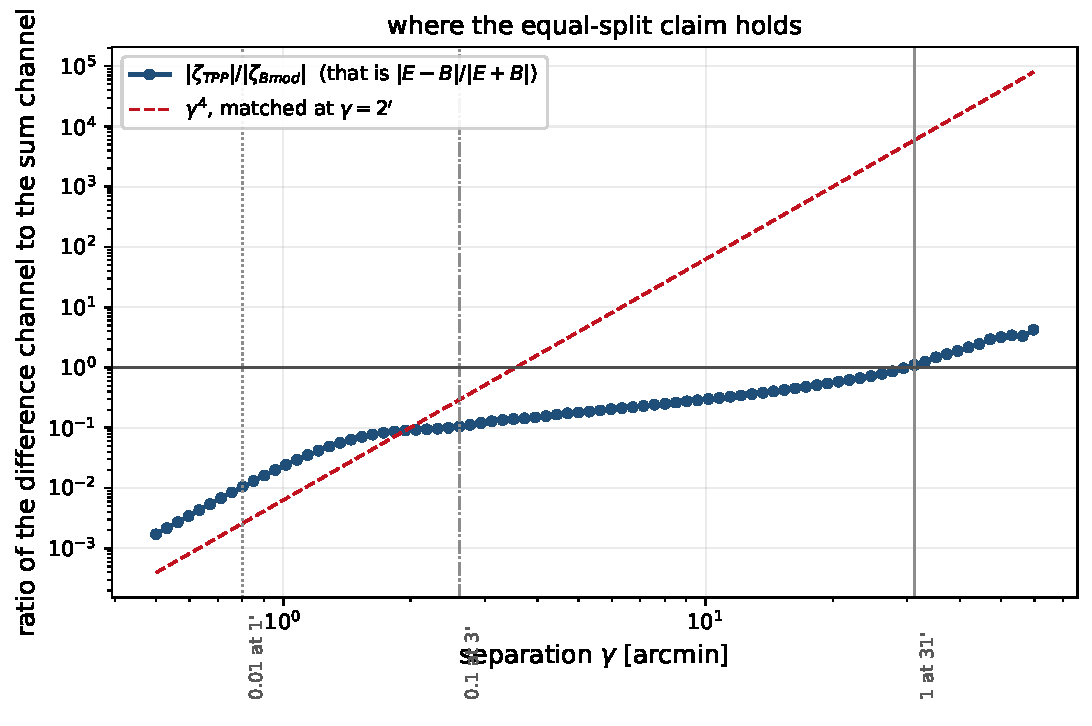
\includegraphics[width=0.78\textwidth]{figures/eb_structure.pdf}
\caption{The ratio of the difference channel $\zeta_{TPP}$, which carries
$C_\ell^{EE}-C_\ell^{BB}$, to the sum channel $\zeta_{Bmod}$, which carries
$C_\ell^{EE}+C_\ell^{BB}$, on the source shell. The dashed line is a
$\gamma^4$ reference matched at $2'$. Beyond about $60'$ the sum channel
passes through zero and the ratio stops being meaningful, so the plot
stops there. Produced by \code{code/rebuild/fig\_eb\_structure.py}.}
\label{fig:eb}
\end{figure}

\subsection{What the corrected calculation gives}

With the vertex resolved, $\xi_-$ is no longer at the numerical floor and
the two polarizations no longer carry equal power. In the corrected run,
after the callable corrections of Section~\ref{sec:callablefix},
$\max|\Delta C_\ell^{EE}|=1.69\times10^{-6}$ and
$\max|\Delta C_\ell^{BB}|=7.03\times10^{-7}$, so $B/E\simeq0.42$ in power
rather than $1$. \emph{Superseded}: a ratio of two maxima is not a stable
number, because the two maxima sit at different multipoles and both sit in
the low-$\ell$ region that Section~\ref{sec:afterwards} shows is not
converged. Taken over $\ell\ge2$ it reads $1.57$, over $\ell\ge20$ it
reads $0.54$. The stable statement is per multipole, over the converged
band: $\Delta C_\ell^{BB}/\Delta C_\ell^{EE}$ falls from $0.95$ at
$\ell=60$ to $0.42$ at $\ell=1500$, median $0.63$. Against the Order-0 $E$-mode band power that is a B-mode
contribution of a few tenths of a percent.

The permutation caveat that an earlier version of this number carried is
gone: $\xi_-$ is carried by the spin channels, which were the ones the
symmetrised tensor fill mishandled, and correcting it moves $B/E$ from
$0.36$ to $0.42$. What remains is the cutoff of Section~\ref{sec:cutoff},
which raises the whole FK term; the ratio is more robust than the
amplitude.

That a B-mode exists at all is not surprising at this order, and it is the
part worth keeping: an Order-2 term sourced by driving-field
non-Gaussianity generates shear B-modes, and B-modes are the standard null
test in cosmic shear. A prediction at the few tenths of a percent level is
small, but it is a prediction, and the draft currently states a different
one.

\subsection{The parity null is a theorem, not a measurement}

$C_\ell^{EB}$ is exactly zero in the corrected run, as in the deployed one.
This survives, and the reason should be stated plainly. Under a reflection
about the separation axis $\Phi_{00}\to\Phi_{00}$, $\Psi_+\to\Psi_+$ and
$\Psi_\times\to-\Psi_\times$, so $\langle\Phi_{00}\Psi_+\Psi_\times\rangle$
equals minus itself and vanishes. The implementation encodes this
structurally: every coupling-tensor entry with an odd number of index-2
slots is never assigned and stays zero, and the tabulated channels carry
only the real parts that populate the even entries.

The consequence is that the parity panel of the draft's
$C_\ell^{EB}$ figure is not an independent numerical test of parity in the
driving field. The input has $C_\ell^{EB}=0$ by construction. What the
figure does demonstrate, usefully, is that the curved-sky transform and the
fold do not leak $E$ or $B$ power into $EB$ at any level above the
numerical floor. That is worth saying, and it is a different statement from
the one a reader would infer.

\subsection{Recommended wording}

\begin{itemize}
\item Keep: the $\gamma^4$ suppression of $\xi_-$, which is measured to
hold with slope $4.00$ at small separation.
\item Keep: $C_\ell^{EB}=0$, stated as a parity theorem and as a check on
the transform rather than as a measurement of the driving field.
\item Replace: ``the FK power splits equally between the two
polarizations, $\Delta C_\ell^{EE}=\Delta C_\ell^{BB}$'' by a statement
that the split is equal in the coincident limit and that away from it the
two polarizations separate, the B-mode falling from $0.95$ of the E-mode
power at $\ell=60$ to $0.42$ at $\ell=1500$. The ``reaches the size of the
sum near $20$ arcminutes'' form of this item was measured at the deployed
cutoff and does not survive: at the converged cutoff $\xi_-/\xi_+$ is
$0.21$ at $22'$ and does not approach unity until about a degree.
\item Replace: ``FK cancels below the plotted floor'' in $\xi_-$ and
$\xi_{\kappa\gamma_t}$ by the corrected magnitudes, with the permutation
caveat attached.
\end{itemize}

\section{Does a nonlinear bispectrum give a more realistic prediction?}
\label{sec:nonlinear}

This is the question the programme started from. The comparison run here is
tree level against BiHalofit, on the corrected grid, as a function of the
multipole cutoff, so that the model change and the convergence question are
not confounded. The answer separates into three parts that do not move
together.

\subsection{Shape: it does move, and this was expected to be the settled part}

The working expectation before the measurement was that the angular shape
would be settled: fixed by how the collapsed three-point cumulant decays
with transverse separation, and insensitive to the cutoff and to the
bispectrum model. That is not what the measurement shows, and it is worth
being explicit because it was the part assumed safe.

Normalising each curve to its own value at $0.5'$ and comparing over
$0.5'$ to $114'$:

\begin{center}
\begin{tabular}{lr}
\toprule
comparison & largest shape change \\
\midrule
BiHalofit against tree, both at $\elmax=960$ & $32\%$ \\
tree at $\elmax=7680$ against $\elmax=960$   & $62\%$ \\
tree at $\elmax=15360$ against $\elmax=960$  & $75\%$ \\
\bottomrule
\end{tabular}
\end{center}

The shape narrows as the cutoff rises. At $\gamma=13.6'$ the normalised
curve reads $0.44$ at $\elmax=960$ and $0.17$ at $\elmax=15360$. That
direction is physically sensible rather than alarming: a higher cutoff
admits shorter-wavelength modes, which decorrelate over shorter
separations, so the angular correlation narrows. The nonlinear model
narrows it slightly further at fixed cutoff, for the same reason.

What survives is the qualitative shape statement rather than a quantitative
one: the FK term decays monotonically with separation across the plotted
range, at every cutoff and for both bispectrum models, and it does so
without the flat plateau the deployed sampling produced. The rate of that
decay is not settled and should not be quoted as if it were.

\subsection{Amplitude: it does not converge to anything}

\begin{table}[h]
\centering
\begin{tabular}{rrrrrr}
\toprule
$\elmax$ & tree & BiHalofit & ratio & tree/O0 & hard $k$, near shell \\
\midrule
960 & $4.080\times10^{-6}$ & $6.603\times10^{-6}$ & 1.619 & 0.48\% & 7\,$h$/Mpc \\
1920 & $8.160\times10^{-6}$ & $21.630\times10^{-6}$ & 2.651 & 0.97\% & 13\,$h$/Mpc \\
3840 & $12.928\times10^{-6}$ & $67.662\times10^{-6}$ & 5.234 & 1.53\% & 26\,$h$/Mpc \\
7680 & $17.080\times10^{-6}$ & $181.821\times10^{-6}$ & 10.645 & 2.02\% & 52\,$h$/Mpc \\
15360 & $19.500\times10^{-6}$ & $347.230\times10^{-6}$ & 17.806 & 2.31\% & 105\,$h$/Mpc \\
\bottomrule
\end{tabular}
\caption{The FK contribution to $\xi_\kappa$ at $\gamma=0.5'$, tree level against BiHalofit, on the corrected grid, as a function of the multipole cutoff. Order-0 there is $8.443\times10^{-4}$. The last column is the largest wavenumber the bispectrum is asked for at the innermost shell; BiHalofit is calibrated to $k\lesssim10\,h$/Mpc. Produced by \code{code/rebuild/table\_nonlinear.py}.}
\label{tab:nonlinear}
\end{table}


This is sharper than expected, and it is the result that decides the
question. At the deployed cutoff the nonlinear bispectrum multiplies the
arcminute FK amplitude by $1.6$. That factor then grows with the cutoff
without settling: $2.7$, $5.2$, $10.6$, $17.8$ at
$\elmax=1920$, $3840$, $7680$, $15360$.

The tree-level and nonlinear cases behave qualitatively differently
(Figure~\ref{fig:cutoff}, middle panel). The tree curve flattens: its
successive increments are $2.00$, $1.58$, $1.32$, $1.14$, so it is
converging, toward roughly $2.5\%$ of Order-0. The BiHalofit curve does
not: its increments are $3.28$, $3.13$, $2.69$, $1.91$, and by
$\elmax=15360$ the FK term has reached $41\%$ of the Order-0 signal.

A term that is $41\%$ of the signal it corrects is not a perturbative
correction, and that number should not be read as a prediction. The reason
is structural rather than a matter of insufficient effort, and
Section~\ref{sec:uv} sets it out: the quantity being computed is a
coincident-point moment of a point-like beam, which has no finite value for
a nonlinear input. The cutoff is acting as an unstated regulator, so the
$41\%$ is a property of where the sum was stopped.

\subsection{Trustworthiness: the honest answer is negative}

Two separate limitations, and neither is removed by a better emulator.

\paragraph{BiHalofit is not independent of perturbation theory.} Its
three-halo term is built on the tree-level $F_2$ kernel with a fitted
effective spectrum. Only the one-halo term carries genuinely new,
simulation-calibrated information. So swapping tree for BiHalofit measures
how much the FK term grows once small-scale nonlinear power is included. It
does \emph{not} provide an independent check that the tree-level
calculation was right. The same holds for a bacco-style emulator: it shares
the gravity backbone and the whole projection chain.

\paragraph{The growth is concentrated at the lensing-kernel peak.} It is
worth asking which shells drive it, because the answer is not the obvious
one. Between $\elmax=960$ and $15360$ the tree vertex grows most at the
outer shells, by a factor $15$ at the source shell and only $1.5$ at the
innermost one: at the innermost shell the linear spectrum is already steep
enough that the integral had converged by $\elmax=960$. The nonlinear
vertex behaves differently, growing by a factor $69$ at
$\chi=3414$ Mpc, against $19$ at the source shell and $11$ at the
innermost. That intermediate shell is near the peak of the lensing
efficiency, and the wavenumber it reaches at the top cutoff is
$13\,h/$Mpc, which is exactly where the one-halo term flattens the spectrum
most. So the nonlinear growth is not confined to a corner of the integral
that the lensing kernel suppresses; it sits where the kernel is largest,
which is why the folded amplitude grows faster than the vertex at any
single shell.

\paragraph{And it happens where the model is not calibrated.} The last
column of the table is the largest wavenumber the bispectrum is asked for
at the innermost shell. At $\elmax=960$ it is $6.6\,h/$Mpc, inside
BiHalofit's calibration, and the factor $1.6$ measured there is a
defensible bound on the bispectrum-model contribution to the FK error
budget. By $\elmax=1920$ it is $13\,h/$Mpc, already outside. By $15360$ it
is $105\,h/$Mpc, which is inside single haloes, an order of magnitude
beyond the calibration and far into the regime where baryonic feedback
rather than gravity sets the matter spectrum. So the factor is trustworthy
exactly where it is smallest, and stops being trustworthy as it grows.

\subsection{The answer, in one sentence}

A nonlinear bispectrum gives a more realistic \emph{input} and an answer
that is not defined: the tree-level FK term converges to about $2.5\%$ of
Order-0 because the linear spectrum is steep enough to make the
coincident-point moment finite, while the nonlinear one has no limit
without a smoothing scale the formalism does not supply
(Section~\ref{sec:uv}), reaching $41\%$ of Order-0 at a cutoff where its
dominant modes sit at $100\,h/$Mpc. The defensible presentation is the
amplitude as a function of the small-scale cutoff, with the model
comparison quoted only where the cutoff keeps the dominant modes inside the
calibrated range, which is the deployed cutoff and not much beyond it.

This is a negative answer to the question the programme started from, and
it is worth stating as such rather than as a caveat attached to a quoted
nonlinear number.

\subsection{What would actually validate the model}

Neither BiHalofit nor an emulator can, for the reason above. Two things
could, and neither has been done:

\begin{enumerate}
\item A convergence-bispectrum comparison: predict
$B_\kappa(\ell_1,\ell_2,\ell_3)$ with the same machinery and compare
against direct measurements on public ray-traced lightcones. This tests the
Poisson factor, the screen-Hessian normalisation, the Limber projection and
the measure together. It cannot reach the coincident limit the FK term
samples, so it does not close the gap, but nothing available gets closer.
\item A direct measurement of the collapsed three-point cumulant of the
driving fields on N-body lightcones, which does close it.
\end{enumerate}

\section{Why the nonlinear case does not converge, and what that means}
\label{sec:uv}

Section~\ref{sec:cutoff} reports that the tree-level vertex converges near
$\ell\sim10^4$ while the nonlinear one does not, and Section~\ref{sec:nonlinear}
reports that the nonlinear FK term reaches $41\%$ of Order-0 at the highest
cutoff tried. Phrased as ``not converged'', that invites the response that
the calculation was not carried far enough. It was not a matter of carrying
it further, and the distinction matters for what the draft should claim.

\subsection{Where the sensitivity comes from}

The FK term samples the driving-field three-point cumulant in the collapsed
configuration, with two of the three legs at the same point on the ray. A
cumulant with coincident legs is a variance-like object, and variances of
cosmological fields are dominated by the smallest scales retained. This is
the same statement as the nonlinear density variance depending on its
smoothing scale, and it is a property of the quantity rather than a defect
of the calculation.

After the Limber radial collapse the hard pair contributes as a
two-dimensional transverse integral $\int\!\mathrm{d}k\,k\,P(k)$, whose
integrand goes as $k^{1+n_{\rm eff}}$: it peaks where $n_{\rm eff}=-1$ and
converges once $n_{\rm eff}<-2$. Measured on the fiducial spectra at $z=1$:

\begin{center}
\begin{tabular}{rrrrr}
\toprule
$k$ [$h$/Mpc] & $n_{\rm eff}$ linear & $1+n_{\rm eff}$ & $n_{\rm eff}$ halofit & $1+n_{\rm eff}$ \\
\midrule
0.1 & $-1.67$ & $-0.67$ & $-1.60$ & $-0.60$ \\
1.0 & $-2.29$ & $-1.29$ & $-1.15$ & $-0.15$ \\
10  & $-2.61$ & $-1.61$ & $-2.08$ & $-1.08$ \\
100 & $-2.77$ & $-1.77$ & $-2.39$ & $-1.39$ \\
\bottomrule
\end{tabular}
\end{center}

The linear spectrum crosses $-2$ at $k=0.21\,h$/Mpc, so the tree-level
integral has a finite limit: $50$, $90$ and $99\%$ of it lie below $k=0.61$,
$8.6$ and $85\,h$/Mpc. The one-halo term flattens the nonlinear spectrum so
that it crosses $-2$ only at $k=8.4\,h$/Mpc, and at $k=1$ it sits at
$n_{\rm eff}=-1.15$, which is essentially the peak of the integrand: every
decade then contributes comparably, and $50$, $90$ and $99\%$ of the
integral lie below $k=9.6$, $80$ and $179\,h$/Mpc.

\subsection{It is not the Limber approximation}

Two things point the same way. The coincident-leg structure exists before
any Limber approximation is made, so the sensitivity is not introduced by
it. And Limber replaces a three-dimensional hard-mode integral by a
two-dimensional transverse one, relaxing the convergence condition from
$n_{\rm eff}<-3$ to $n_{\rm eff}<-2$; dropping Limber would therefore make
the divergence worse, not better. Limber's own failure mode is at low
multipole and wide angle, which is a different regime from this one.

\subsection{What is actually missing}

The formalism as written carries no smoothing scale. A search of
\code{sections/} finds no beam width, no coarse-graining, and $\elmax$ does
not appear in the text at all: it exists only in the code. So the quantity
being computed is a coincident-point moment of a mathematically point-like
beam, and that quantity has no finite value for a nonlinear input. The
cutoff is acting as an unstated regulator that sets the answer.

The tree-level case escapes this because it happens to be ultraviolet safe,
so no regulator is needed and the number is well defined. That is the
regime the draft is in, and nothing here undermines it. What does not
follow is that the same calculation can be upgraded to a nonlinear input by
substituting a better bispectrum.

\subsection{A finite beam would supply the missing scale}

The physical candidate is that a real beam has finite cross-section, so the
driving fields entering the Sachs system are averages over that section
rather than point values. The algebra of that proposal is worked out in
\code{SFT-lensing-paper-analyses/mathematica/beam\_width\_regulator.wl},
15 checks, all passing. What it establishes:

\begin{itemize}
\item For a normalised axisymmetric screen-plane window of width $s_b$,
averaging gives
$\bar\Phi = \Phi + (s_b^2/4)\,\nabla^2_\perp\Phi + O(s_b^4)$, and in Fourier
space it is multiplication by $\tilde W(k)=\exp(-k^2s_b^2/4)$, whose
small-$k$ expansion reproduces the same coefficient.
\item An axisymmetric window does not mix spin weights, so $\Phi_{00}$ stays
spin 0 and $\Psi_0$ stays spin 2 under averaging. The projection of
$e^{is\theta}$ against such a window vanishes for every $s\ne0$.
\item The windowed transverse integral converges for \emph{any} power-law
spectrum, because $\tilde W^2$ decays faster than any power. At the halofit
slope $n_{\rm eff}=-1.15$ the unwindowed integral diverges and the windowed
one is finite.
\item The window suppresses modes above $k\sim2/s_b$, so with the Limber map
it fixes $\elmax = 2\chi_h/s_b$. A beam of $1\,h^{-1}$Mpc gives
$\elmax\simeq590$ at the innermost shell and $11\,000$ at the source shell;
a beam of $3\,h^{-1}$Mpc gives $200$ and $3700$.
\end{itemize}

So the proposal does what is needed: it removes the divergence, and it
replaces a free cutoff by a scale that is a property of the observation.

\subsection{What the script does not settle}

Two limitations, both recorded in the script rather than left implicit.

It does not establish that beam averaging is the correct definition of this
observable, nor which scale to use. Candidates differ by orders of
magnitude: the angular size of the source, the resolution element of the
instrument, and the smoothing applied to the convergence map are all
defensible readings and give very different $\elmax$. That is a choice
about what is being measured, and it has to be made before a nonlinear
number can be quoted.

And averaging the drivers is not the same operation as solving for a finite
beam. The Sachs system is nonlinear in the optical scalars, so averaging
does not commute with the quadratic terms; the bundle variance survives,
and the two differ at second order in the optical scalars. Beam averaging
therefore defines the source, and a genuine finite-beam treatment would be
a further step.

\subsection{Consequence for the draft}

The presentation that follows from this is not ``the FK amplitude is
$X$, subject to a cutoff''. It is:

\begin{itemize}
\item the tree-level FK term is well defined and converges, to about
$2.5\%$ of Order-0 at arcminute separations, five times the value the draft
quotes at the deployed cutoff;
\item a nonlinear FK amplitude is not defined without a smoothing scale,
and the formalism does not currently supply one;
\item quoting a nonlinear number therefore requires either adopting a beam
width as part of the observable's definition, or an effective-theory
treatment in which the ultraviolet-sensitive part is absorbed into a
counterterm fixed by simulation or data.
\end{itemize}

\section{What changes in the draft}
\label{sec:draft}

Statements are grouped by whether the measurements support them. Nothing in
\code{sections/} was edited; this is a list, not a patch.

\subsection{Statements that survive}

\begin{itemize}
\item The arcminute FK amplitude. \code{insights.tex} line~193: ``at small
separation, FK reaches a few $\times10^{-6}$, about $0.5\%$ of Order-0 and
roughly twice the FF term''. Corrected: $+4.28\times10^{-6}$, $0.51\%$ of
Order-0, $2.1$ times FF. This is the number the draft leans on most and it
is unaffected, because at $0.5'$ the queried configuration really does sit
on the tabulated corner.

\item The selection rule and its mechanism. \code{insights.tex} lines
188--192, that FK concentrates in the modulus pair $\xi_\kappa$ and
$\xi_+$ and is suppressed in the other two. The corrected calculation
preserves the ordering: FK is $0.5$ to $1\%$ of Order-0 in the modulus pair
and $0.5$ to $0.8\%$ in the other two, having been $10^{-16}$ to $10^{-9}$
there before. The rule is a statement about which combinations FK enters
strongly, and that survives; the claim that it vanishes does not.

\item The channel algebra of \code{conclusion.tex} lines 50--58, that
$\xi_+$ is sourced by the sum
$\langle\Phi_{00}\Psi_+\Psi_+\rangle+\langle\Phi_{00}\Psi_\times\Psi_\times\rangle$
and $\xi_-$ by the difference. That is a statement about the vertex
structure and is untouched.

\item Figure~7, the driving-field $\zeta$ slices. It is built from
$\gamma$-resolved data and is correct as printed.

\item The parity null. $C_\ell^{EB}$ remains zero identically in the
corrected run, as it must by parity.

\item The Monte-Carlo validation, read as the draft states it: ``with the
input statistics held fixed''. It validates the diagram assembly. It is
structurally blind to this error, because it reads the same table.
\end{itemize}

\subsection{Statements that do not survive}

\begin{itemize}
\item \code{insights.tex} lines 194--196: FK ``overtakes the falling
Order-0 signal beyond $\sim2^\circ$''. There is no crossover. The corrected
ratio is flat at $0.5$ to $1\%$ across the whole range.

\item \code{insights.tex} lines 119--122, the caption of the draft's
two-point decomposition figure: ``overtakes Order-0 in absolute
amplitude beyond $\gamma\sim2^\circ$''. Same artefact.

\item \code{insights.tex} lines 196--199: in $\xi_-$ and
$\xi_{\kappa\gamma_t}$, ``FK drops to the numerical floor''. It does so at
$\gamma\to0$ only. At the plotted separations the corrected FK is $0.5$ to
$0.8\%$ of Order-0 in both.

\item \code{insights.tex} lines 202--204 and the caption of the
$C_\ell$ figure: ``the $\gamma$-flat FK term shows up as a low-$\ell$
excess''. The flatness is the interpolation weight. The excess, a factor 18
over Order-0 at $\ell=3$, becomes $-0.20$ with a resolved vertex; FK
instead appears as a steady $0.8\%$ correction over $39\le\ell\le800$.

\item \code{conclusion.tex} lines 34--36: the leakage ``lifts the
convergence and the parity-even shear at the few-percent level and
overtakes the linear signal in absolute amplitude beyond roughly
$2^\circ$''. The lift is a few tenths of a percent to one percent, not a
few percent, and there is no crossover.

\item \code{conclusion.tex} lines 60--62: ``The FK power therefore splits
equally between the two polarizations,
$\Delta C_\ell^{EE}=\Delta C_\ell^{BB}$''. The isotropy argument that
supports it is exact at zero separation, where $\Psi_+$ and $\Psi_\times$
are statistically equivalent. At finite separation the separation vector
picks out an axis and they are not, so the equality does not extend to the
plotted range. In the corrected run
$\max|\Delta C_\ell^{EE}| = 1.69\times10^{-6}$ against
$\max|\Delta C_\ell^{BB}| = 7.03\times10^{-7}$, that is $B/E\simeq0.42$ in
power.

\item \code{conclusion.tex} lines 133--136: ``the large-angle FK excess
sits at low multipoles ($\ell\lesssim10$)''. There is no large-angle
excess. The surrounding caveat about the relativistic Poisson source and
the observed-redshift correction remains worth making, but it is no longer
attached to a feature in the data.

\item \code{appendix.tex} lines 601--603, the caption of the validation
figure: ``FK its decay toward the sign change at $\gamma\simeq32^\circ$''.
That is where the four-neighbour set drops the $(1,1,1)$ node. It is an
interpolation switch described as physics.

\item \code{conclusion.tex} line 36: the leakage ``strengthens steadily
with source redshift''. This is not refuted here, it is untested. Two
separate effects bias it in exactly that direction, and both are addressed
in Section~\ref{sec:lambdamin}.
\end{itemize}

\subsection{Figures that must be replaced}

Six of the sixteen figures depend on the vertex.

\begin{table}[h]
\centering
\begin{tabular}{llp{6.6cm}}
\toprule
\# & figure & status \\
\midrule
2 & \code{analysis3\_NLO\_FFFK.pdf} & regenerated; FK no longer crosses
Order-0, and the two lower panels now carry a visible FK curve \\
3 & \code{analysis3\_cl\_full\_vs\_O0.pdf} & regenerated; the low-$\ell$
excess is gone \\
4 & \code{cl\_EB\_polarization.pdf} & regenerated; $EE$ and $BB$ no longer
coincide, $EB$ still zero \\
5 & \code{multiz\_kappa\_xi\_cl.pdf} & needs regeneration; its cached FK
slice comes from the same table. The corrected redshift dependence it
should show is measured in Section~\ref{sec:lambdamin} and plotted in
Figure~\ref{fig:redshift}, including the $\lammin$ bias on its lowest
slice \\
6 & \code{appendix\_mc\_workflow.pdf} & its FK curve moves with the
corrected table, but the agreement it demonstrates does not, because the
Monte-Carlo reads the same vertex through \code{driver\_stats.py} and both
sides move together. Regenerating it re-plots the corrected values; it does
not test the correction. Its caption separately needs the $32^\circ$
sentence removed, since that feature is the interpolation-weight zero \\
7 & \code{zeta\_driving\_field\_slices\_draft.pdf} & unchanged as printed,
being built from resolved data. Worth re-examining only for the cutoff
question of Section~\ref{sec:cutoff} \\
\bottomrule
\end{tabular}
\caption{The vertex-dependent figures. Figures 1 and 8 to 16 do not depend
on the vertex and are unaffected.}
\label{tab:figures}
\end{table}

Two cautions carried over from the figure manifest. The generator for
Figure~7 writes directly into the repository \code{figures/} directory with
a hardcoded path, so it overwrites the paper's file if run. Figure~5
depends on an external cache under \code{talk/}, so its FK slice must be
regenerated rather than reused. The regenerations here were produced by
\code{code/figures\_corrected/regenerate.py}, which imports each paper
generator, rebinds only its FK input and output paths, and calls its
\code{main()}. The plotting, styling and observable definitions are
therefore the paper's own, unmodified, and nothing was written into
\code{figures/}. The regenerated files are in
\code{driver\_field\_emulators/figures/corrected/}, named after the
generator's own output stem. The \code{\_permfix} versions are the ones to
use: they carry both the grid correction and the callable corrections of
Section~\ref{sec:callablefix}. The \code{\_corrected} versions carry the
grid correction only and are kept for comparison.

\section{What remains uncertain}
\label{sec:uncertain}

\subsection{Open, and quantified}

\paragraph{The permutation handling of the spin channels.} Measured in
Table~\ref{tab:perm} and now fixed, see Section~\ref{sec:callablefix}. It
is listed here because the residual is not zero: the corrected lookup
requires the table to be closed under the leg permutations it queries, and
while the production mesh and the densified collapsed family both are, a
table built without that closure would fall back silently. The callable
checks the closure at load and warns.

\paragraph{The angular floor of the lookup.} Fixed, see
Section~\ref{sec:callablefix}. It was a floor at $\gamma = 0.344'$ against
a smallest plotted separation of $0.5'$, so the published points survived
it by about a factor two, but ten of the 157 refined collapsed nodes were
being absorbed by it. The floor is now $0.0034'$ and the refinement is no
longer capped by the callable.

\paragraph{The source redshift label.} All three production runs use
\code{t\_final = 2313.0289} Mpc, described everywhere as $z_s = 5$. On the
vertex table's own $\lambda\leftrightarrow z$ mapping that affine distance
is $z = 4.70$; $\lambda(z{=}5)$ is $2317.96$ Mpc. The three runs share the
value, so every comparison between them is internally consistent and no
conclusion here is affected, but the quoted source redshift and the value
used do not correspond. It is worth reconciling before the numbers are
quoted again.

\subsection{Open, and not quantified here}

\paragraph{The collapsed corner of the vertex.} The absolute normalisation
of the transfer chain is no longer open: Section~\ref{sec:normalisation}
shows it reduces to the standard Limber convergence bispectrum exactly.
What that argument cannot reach is the coincident configuration the FK term
actually samples. A measured convergence bispectrum lives on resolvable
triangles with a finite soft leg, and the analytic assembly is a statement
about the projection rather than about the driving-field cumulant at zero
separation. Closing this needs a direct measurement of the collapsed
three-point cumulant of the driving fields on N-body lightcones, which
nobody has done. The existing internal checks cannot substitute: the
Order-0 comparison against PyCCL validates the two-point chain and never
touches the three-point vertex, the \code{fastnc} closure test covers open
triangles only, and the Monte-Carlo cross-check reads the same table as the
production fold.

\paragraph{The empirical anchor was not turned into a ratio.} The
comparison against the published ray-traced measurement in
Section~\ref{sec:normalisation} confirms the prediction lies in the right
decade with the right shape, but quoting a ratio needs the digitised
measurement points. That is the one part of the specified normalisation
study left undone.

\paragraph{The smoothing scale of the observable.} This is now the sharpest
open question, and Section~\ref{sec:uv} states it. The FK term samples a
coincident-point moment, which is finite for the linear spectrum and not
for a nonlinear one, and the formalism carries no scale that would make it
finite. Beam averaging supplies one, and its algebra checks out, but which
physical scale to adopt is undetermined: the source's angular size, the
instrument's resolution element and the smoothing of the convergence map
differ by orders of magnitude and give correspondingly different cutoffs.
Until that is settled, no nonlinear FK amplitude can be quoted. The
tree-level amplitude is unaffected.

\paragraph{Finite-beam optics beyond averaged drivers.} Averaging the
drivers is not the same as solving the Sachs system for a beam of finite
width, because the system is nonlinear in the optical scalars and averaging
does not commute with the quadratic terms. The difference is second order
in the optical scalars and has not been evaluated.

\paragraph{Cross-shell against equal-shell.} The tabulated vertex is
equal-shell by construction. The error made by collapsing the cross-shell
cumulant onto equal shells scales as $O[(\Delta\chi/\chi_s)^2]$ under
Limber, which is the justification the draft gives, and it has not been
measured directly.

\paragraph{Wide angles.} Beyond about $1500'$ every curve here is at the
cancellation floor and changes sign. Ratios in that region carry no
information and none is quoted.

\section{Findings that came later}
\label{sec:afterwards}

The sections above were written before the revision was carried out. Four
things were found while carrying it out, each of which changed what was done.
They are recorded here rather than folded into the earlier sections, so that
the order in which the evidence arrived stays legible.

\subsection{The FK Monte-Carlo does not measure the FK diagram}

Section~\ref{sec:sampling} treats the appendix Monte-Carlo as a check that
could not have caught the interpolation error, because it reads the same
tabulated cumulant. That is true, but it understates the situation. With the
corrected vertex the Monte-Carlo points depart from the analytic channel by a
factor two at $2'$ and carry the wrong sign beyond $6'$, which sent us to the
estimator itself.

Its expectation can be computed exactly at the diagram's order, by pure linear
algebra with no realisations, and doing so reproduces all $21$ probe points to
about $1.5$ seed standard errors. It decomposes into two terms, neither of
which is the FK diagram. First, the variance-reduced estimator injects the
third cumulant only on the observable-side leg of the vertex, so of the three
placements that make up $\zeta = Q\!:\!VV + \text{perms}$ it captures one; in
the eigenbasis of the node covariance the captured fraction is
$d_q d_r/(d_p d_q + d_q d_r + d_r d_p)$, which kernel-weighted comes to
$0.245$ at $0.5'$, passes through zero near $10'$ and is negative beyond.
Second, a finite-$\sigma_\lambda$ term enters because the AR(1) smearing
decoheres the node-local vertex from the smeared covariance, releasing the
cancellation of the tabulated tensors' $\lambda$-grid graininess; smoothing
both tensors makes the model $\sigma_\lambda$-flat at exactly the share
prediction, which is the attribution.

The historical agreement at $\sigma_\lambda=8$ was these two errors summing
through unity at a value that had itself been chosen so that the ratio came
out one. The FK amplitude also scales close to linearly with
$\sigma_\lambda$ ($8.70$, $19.8$ and $37.9\times10^{-6}$ at $0.5'$ for
$\sigma_\lambda=4,8,16$), with an intercept consistent with zero, so no range
of that estimator is a converged measurement of FK.

The FK points were therefore withdrawn from the figure. The channel is now
checked by a direct quadrature contraction of the tabulated cumulant with the
FK kernel,
\[
  \mathrm{FK}(\gamma) = 2\!\int\!\mathrm{d}v\, W(v)\,H(v)\,
     \Bigl[-\!\sum_c \zeta^{(6)}_{cc B}(\gamma; v)\Bigr],
  \qquad
  H(v) = D(v)^4\!\!\int_v^{\lambda_s}\!\!\frac{W(u)}{D(u)^4}\,\mathrm{d}u ,
\]
which shares only the vertex table with the workflow and reproduces the folded
channel to $0.99$--$1.02$ over $0.5'$--$5'$ and $1.07$ at $17.3'$. The FF
channel keeps its Monte-Carlo points: FF is a term in the equation of motion
and can be differenced at a fixed random draw, so its noise scales with the
effect itself, whereas a third moment measured from realisations scatters
according to the Gaussian fluctuations of the field however small the cumulant
is.

\subsection{The multi-redshift FF slices had never been computed}

The apparent low-$\ell$ excess at $z_s=1.7$ in the multi-redshift figure was
not physics and not the interpolation error either. The cache filled the FF
slices at $z_s<5$ with the exact $z_s=5$ result scaled by the \emph{per-%
$\gamma$} ratio $f_K(z)/f_K(5)$. At large separation $f_K$ sits on its
numerical floor, so that ratio is noise over noise: the tails carried
$10^{-7}$-level dips and went negative at $z_s=1$, which the FF moment cannot
do, being a connected part plus $\langle\kappa\rangle^2>0$. Through the
truncated-range transform this became an excess of order the Order-0 signal.

Five genuine per-redshift sweeps were run in its place, one single-threaded
process per source distance, about $3.2$ hours each. Two checks: each slice's
large-separation plateau matches the deterministic $\langle\kappa\rangle^2(z_s)$,
obtained by propagating the expectation of the same recursions with no
Monte-Carlo, to $1.022$, $1.005$, $1.005$, $0.999$ and $1.008$ at
$z_s=1,\,1.7,\,2.5,\,3.2,\,4$; and a $z_s=5$ control, run the same way with
fresh caches, reproduces the production FF \emph{bit-identically} at all forty
separations. The production path is a real computation, deterministically
reproducible, and this is the same path.

\subsection{The multipole sum stops converging beyond about a degree}

Separation enters the cumulant only through $P_{\ell_3}(\cos\gamma)$. That
factor is unity for every term at coincidence, so the sum is coherent there
and each doubling of the cutoff adds to it. Once $\ell_3\gamma\gtrsim1$ it
instead oscillates with period $\Delta\ell_3=2\pi/\gamma$ and is damped as
$(\ell_3\gamma)^{-1/2}$, so the high-multipole terms alternate in sign and
largely cancel. The low-multipole branch, where $\ell_3\gamma\ll1$, stays
almost constant: measured on the $z=5.7$ shell, $\zeta_{TTT}$ for $\ell\le60$
is $+1.33\times10^{-16}$ at every separation, while the $\ell>60$ part falls
from $-3.7\times10^{-13}$ at $0.5'$ to $-1.5\times10^{-16}$ at $232'$. The two
necessarily cross, and near the crossing $\zeta$ is a small difference of two
comparable numbers computed by different methods.

Three independent symptoms follow, and all three place the boundary near a
degree. Two evaluations of the same multipole sum, one wide window against
eight disjoint ones, agree to $3$--$6\%$ below $85'$ and differ by factors of
several to several tens beyond $117'$. Two independent evaluations of
$\xi_{\rm FK}$, the quadrature above against the workflow fold, agree to
$0.4$--$6\%$ below $20'$ and differ by a factor $5.2$ at $114'$. And raising
the cutoff from $7680$ to $15360$ changes $\xi_{\rm FK}$ by a uniform
$1.08$--$1.14$ for $\gamma\le56'$ but by $0.69$, $0.28$, $2.59$ and $0.73$ at
$114'$, $294'$, $597'$ and $1535'$.

The consequence for the harmonic-space numbers is direct, because low
multipoles are dominated by the large-separation part of the two-point
function. Zeroing $\xi_{\rm FK}$ beyond a cut and re-transforming moves the
$\ell=2$ correction between $-10.9\%$ and $+2.7\%$ as the cut is varied, while
$\ell=100$ stays at $1.14$--$1.24\%$ throughout. FK is therefore quoted only
for $\gamma\lesssim1^\circ$ and $\ell\gtrsim50$, and drawn faint outside that
range.

\subsection{The $\zeta$-slices figure was still at the old cutoff}

It was the last product drawn at $\ell_{\max}=1000$ while everything else had
moved to $15360$, and the cutoff changes the panels rather than only their
normalisation: at the $z=3.1$ shell the peak $|\zeta_{TTT}|$ grows by $13.7$
and the normalised value at $5'$ moves from $-0.87$ to $-0.27$, so the printed
panels showed a cumulant falling about three times more slowly in angle than
the one the numbers come from. Rebuilt at the converged cutoff by appending
four flat-sky Born-Limber windows to $(8000,15360]$, the exact Wigner-3j ladder
staying at $\ell\le60$, and clipped to $\gamma\le85'$ for the reason above.
Its caption also carried a blanket ``change sign with angular scale'' which is
not true at the converged cutoff: within the plotted range $\zeta_{TTP}$ never
changes sign, $\zeta_{TTT}$ and $\zeta_{B}$ change sign at $59'$ only for
$z\gtrsim4$, and $\zeta_{D}$ from $z\simeq1$.


\end{document}
